%compiling with XeLaTeX
\documentclass[twoside,11pt,abstracton]{scrreprt}

% !TeX root = ..//diffgeo_main.tex

%personel data
\title{Differentialgeometrie I}
\author{Dr. Anna Siffert}
\date{Sommersemester 2018}


%math and theorems
\usepackage{amsmath}
\usepackage{amssymb}
\usepackage[amsmath,thmmarks,hyperref]{ntheorem}
\usepackage{mathtools}
\usepackage{dsfont}
\usepackage[arrow, matrix, curve]{xy}
\usepackage{nicefrac}
\usepackage{upgreek}					%Griechische Buchstaben

%language settings and microtype
\usepackage{fontspec} 
\setmainfont{Palatino}
\setsansfont{Optima}
\setmonofont[Scale=MatchLowercase]{Menlo}

\usepackage{polyglossia}
\setmainlanguage{german}
\setotherlanguages{english}
\usepackage{microtype}

%useful packages
\usepackage{geometry}
\usepackage{xcolor}
\usepackage{graphicx}
\usepackage{float}
\usepackage{fancyhdr}
\usepackage{csquotes}
\usepackage{blindtext}
\usepackage{todonotes}
\usepackage{booktabs}
\usepackage{array}
\usepackage[labelfont=bf]{caption}
\usepackage{wrapfig}
\usepackage{physics}
\usepackage{enumitem}

%geometry
\geometry{
	width=150mm,
	bindingoffset=7mm,}

%color settings
\definecolor{myred}{RGB}{196,19,47} 
\definecolor{myblue}{RGB}{0,139,139}


%for empty pages at the beginning of the document
\def\blankpage{%
	\clearpage%
	\thispagestyle{empty}
	\addtocounter{page}{-1}
	\null%
	\clearpage}

% Page layout for beginning of chapter
\fancypagestyle{plain}{%
	\fancyhf{}  % clear all header and footer fields 
	\fancyfoot[C]{- \thepage\hspace{3pt}-} 
	\renewcommand{\headrulewidth}{0pt}
	\renewcommand{\footrulewidth}{0pt}}

%page layout for the other pages
\pagestyle{fancy}
\fancyhf{}
\fancyhead[LE]{\textit{\nouppercase{\leftmark}}}
\fancyhead[RO]{\textit{\nouppercase{\rightmark}}}
\fancyfoot[C]{- \thepage\hspace{3pt}-}
\renewcommand{\headrulewidth}{0.2pt}
\renewcommand{\footrulewidth}{0pt}

% titles and stuff
\setkomafont{chapter}{\normalfont\bfseries\huge}
\setkomafont{section}{\normalfont\bfseries\LARGE}
\setkomafont{subsection}{\normalfont\bfseries\large}
\setkomafont{title}{\normalfont\bfseries\Large}
\setkomafont{author}{\normalfont\bfseries\Large}
\setkomafont{date}{\normalfont\bfseries\Large}

% nice boxes
\usepackage[many]{tcolorbox}    
\newtcolorbox{mybox}[1]{%
	tikznode boxed title,
	enhanced,
	arc=0mm,
	interior style={white},
	attach boxed title to top center= {yshift=-\tcboxedtitleheight/2},
	fonttitle=\large\bfseries,
	colbacktitle=white,coltitle=black,
	boxed title style={size=normal,colframe=white,boxrule=0pt},
	title={#1}}

%proofs,defs ...

%Theorems
\theoremstyle{marginbreak}
\theoremheaderfont{\normalfont\bfseries}
\theorembodyfont{\slshape} 
\theoremseparator{}
\newtheorem{satz}{Satz}[chapter]

%Lemma
\theoremstyle{changebreak} 
\theoremindent0.5cm 
\theoremseparator{}
\newtheorem{lem}[satz]{Lemma}

%Helping lemma, Mathieu, Q's been here
\theoremstyle{changebreak} 
\theoremindent0.5cm 
\theoremseparator{}
\newtheorem{hlem}[satz]{Hilfslemma}

%Corolarys
\theoremindent0cm 
\theoremseparator{}
\newtheorem{kor}[satz]{Korollar}

%Examples
\theoremstyle{break} 
\theorembodyfont{\upshape} 
\theoremseparator{} 
\newtheorem{bsp}[satz]{Beispiel}

%Comments
\theoremstyle{plain} 
\theorembodyfont{\upshape} 
\theoremseparator{:} 
\newtheorem*{bem}[satz]{Bemerkung}

%Definitions
\theoremstyle{break}
\theorembodyfont{\slshape} 
\theoremseparator{} 
\newtheorem{defs}[satz]{Definition}

%Proofs
%\theoremheaderfont{\normalfont} %falls es nicht dick gedruckt sein soll
\theoremstyle{nonumberbreak}
\theoremseparator{} 
\theoremsymbol{\ensuremath{\square}}
\newtheorem{bew}[satz]{Beweis:}

%bibliography
\usepackage[
style=numeric-comp,
backend=biber,
maxnames=10,
maxcitenames=2,
isbn=false,
date=year,
url=false,
doi=false
]{biblatex}
\bibliography{bibliography/diffgeo-bib}

%appendix
\usepackage[toc,page]{appendix}

%killing indent
\setlength{\parindent}{0pt}

%always use hyperref at the end of the preamble!
\usepackage[colorlinks=True]{hyperref}
\hypersetup{allcolors=myred}

% !TeX root = ..//diffgeo_main.tex

% Commands
\newcommand{\R}{\mathbb{R}}	%simplify R^n
\newcommand{\set}[1]{\left\{#1\right\}}	%siplify sets
\newcommand{\difM}{differenzierbare Mannigfaltigkeit}		%abbreveiate "differenzierbare Mannigfaltigkeit"
\renewcommand{\d}{{\operatorname{d}}}		%differentiial operator
\newcommand{\Index}[1]{#1\index{#1}}
\newcommand*{\quelle}[1]{\par\footnotesize Quelle:~\href{#1}{#1}}
\newcommand{\im}{\mathrm{i}}
\newcommand{\e}{\mathrm{e}}
\newcommand{\mfk}{\mathcal{M}}
\newcommand{\mfka}{\mathcal{N}}
\newcommand{\atlas}{\mathcal{A}}
\newcommand{\rn}{\mathbb{R}^n}
\newcommand{\evat}{\vert\big}
\newcommand{\cinf}{C^\infty}
\newcommand{\tspace}[1]{T_{#1} \mathcal{M}}
\newcommand{\covd}{\mathrm{D}}
\newcommand{\curv}{\operatorname{R}}
\newcommand{\tor}{\operatorname{T}}
\renewcommand{\pi}{\uppi}
\renewcommand{\epsilon}{\varepsilon}
\newcommand{\expp}{\operatorname{exp}}

% Operatoren
\DeclareMathOperator{\id}{id} % Identität
\DeclareMathOperator{\supp}{supp} % Support einer Funktion
\DeclareMathOperator{\diff}{Diff} % Menge der Diffeomorphismes
\DeclareMathOperator{\rang}{Rang} % Rang einer Matrix
\DeclareMathOperator{\fix}{Fix} % Fixpunkte 
\DeclareMathOperator{\isom}{Isom} % isometrie
\DeclareMathOperator{\diam}{diam} % Diameter
\DeclareMathOperator{\Jac}{Jac} % Vektorraum der Jacobifelder
\DeclareMathOperator{\injrad}{injrad} % Injektionsradius


\begin{document}
	
%title, abstract and toc	 
\pagenumbering{roman} % start roman numbering before main text
% !TeX root = ..//diffgeo_main.tex
\begin{titlepage}
	\begin{center}
		\makeatletter
		
		\thispagestyle{empty}
		
		\Huge\textbf{\@title} \\
		\vspace{5mm}
		\Large\textbf{ gehalten von \@author} \\
		\large{im \@date} \\
		\vspace{5mm}
		\large{an der} \\
		\Large\textbf{Ruprecht-Karls-Universität Heidelberg} \\
		\vfill
		%\begin{figure}[H]
		%	\centering
		%	\includegraphics*[width=0.6\textwidth]{figures/logo-uni-hd-small}
		%\end{figure}
	    %\vfill
		\Large
		In \LaTeX \ gesetzt von \\ 
		\vspace{3mm}
		\bfseries{
		Thomas Ackermann
		\& 
		Mathieu Kaltschmidt}\\ 	
	   \vspace{2cm}
	   \normalfont
	   aktueller Stand: \  \textit{\today}
		\makeatother
	\end{center}
\blankpage
\end{titlepage}

{\renewcommand{\headrulewidth}{0pt} % kill headrule for abstract and toc
	\addcontentsline{toc}{chapter}{\hspace{.6cm}Vorwort }
	% !TeX root = ..//diffgeo_main.tex
\makeatletter

%\begin{figure}[H]
%\flushright
%\includegraphics[width=0.4\textwidth]{figures/logo-uni-hd}
%\end{figure}
\vspace{-30mm}
\begin{flushleft}	
\textbf{\LARGE\@title} \\
\vspace{0.5cm}
\Large\@author \\
\end{flushleft}
\rule{\textwidth}{0.2pt}

\makeatother

\vfill

{\let\raggedsection\centering
\section*{Vorwort}
Bei diesen Vorlesungsnotizen handelt es sich um kein offizielles Skript, sondern lediglich um die Umsetzung des Vorlesungsmitschriebs in \LaTeX. \\
Für die Vollständigkeit \& Richtigkeit des Inhalts wird deshalb \bfseries keine Gewährleistung \normalfont übernommen. \\
Bei Fragen, Korrekturen und Verbesserungsvorschlägen freuen wir uns über eine Nachricht.\footnote{Mail an \href{mailto:M.Kaltschmidt@stud.uni-heidelberg.de}{M.Kaltschmidt@stud.uni-heidelberg.de}
oder
\href{mailto:T.Ackermann@stud.uni-heidelberg.de}{T.Ackermann@stud.uni-heidelberg.de}	
} \\
Die Dozentin Frau Dr. Siffert empfiehlt die nachfolgende Literatur zur Vertiefung des in der Vorlesung behandelten Stoffs:

% books and more
\nocite{*}
\printbibliography[heading=none]

 Eine Inhaltsübersicht der in der Vorlesung behandelten Themen befindet sich auf der nächsten Seite.

\vfill

\blankpage
	\tableofcontents
	\blankpage}
}
%main content
\setcounter{tocdepth}{1}
\pagenumbering{arabic} % now set main numbering to arabic
\addcontentsline{toc}{part}{\hfill \Large Inhalt der Vorlesung }
%lectures
	% !TeX root = ..//diffgeo_main.tex
\chapter{Differenzierbare Mannigfaltigkeiten}
\section*{Worum geht es in der Differentialgeometrie?}
Die zentralen Objekte der Differentialgeometrie sind Mannigfaltigkeiten. Das Ziel ist es, Analysis und Geometrie auf solchen Mannigfaltigkeiten zu betreiben. \\
Wir beginnen zunächst einmal mit einer kurzen Gegenüberstellung der bereits bekannten Konzepte aus dem $\mathbb{R}^n$ mit den korrespondierenden Begriffen der Differentialgeometrie, welche wir in den kommenden Vorlesungen noch genauer kennenlernen werden.

%Vergleich
\begin{figure}[H]
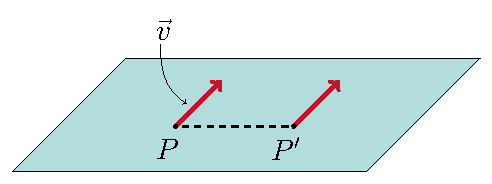
\includegraphics[scale=0.8]{figures/tikz/plane.pdf}
\hspace{2cm}
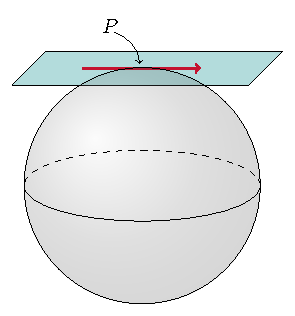
\includegraphics[scale=0.9]{figures/tikz/sphere_with_plane.pdf}
\end{figure}

\begin{figure}[H]
\centering
\begin{tabular}{>{\centering}p{.45\textwidth} | >{\centering}p{.45\textwidth}} 
$\mathbb{R}^n$ \vspace{5pt} & $\Huge\mathcal{M}$  \vspace{5pt} \tabularnewline \hline 
\vspace{5pt} Parallelverschiebung & \vspace{5pt} Begriff des Zusammenhangs\tabularnewline 
\vspace{5pt} Gerade = kürzeste Verbindung & \vspace{5pt} Konzept der Geodätischen \tabularnewline 
\vspace{5pt} flacher Raum & \vspace{5pt} gekrümmter Raum \tabularnewline 
\vspace{5pt} Skalarprodukt & \vspace{5pt} Riemannsche Metrik \tabularnewline 
\end{tabular}
\end{figure}
\section{Definitionen}
Um differenzierbare Mannigfaltigkeiten definieren zu können wiederholen wir zunächst die Definition eines topologischen Raumes. \\
\phantom{.}\\
\bfseries Erinnerung: \normalfont $M \subseteq \mathbb{R}^n$ offen, wenn $\forall p \in U \ \exists \ \varepsilon>0$, sodass $B_{\varepsilon}(p) \subset U$. Dieser Begriff von Offenheit heißt \textit{euklidische Topologie} \normalfont und erfüllt:
\begin{enumerate}
\item[i)] $\emptyset, \mathbb{R}^n$ offen
\item[ii)] $U, V \subset \mathbb{R}^n$ offen $\Rightarrow U \cap V$ offen in $\mathbb{R}^n$
\item [iii)] $U_i, i \in $ I offen in $\mathbb{R}^n \Rightarrow \bigcup\limits_{i \in \text{I}} U_i \subset \mathbb{R}^n$ offen
\end{enumerate} 


\begin{figure}[H]
\centering
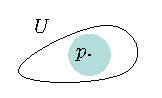
\includegraphics[scale=1.5]{figures/tikz/openset.pdf}
\caption{Offene Menge}
\label{img:offenemenge}
\end{figure} 

\begin{defs}[Topologischer Raum]
Ein topologischer Raum ist eine Menge $X$ zusammen mit einer Menge $\mathcal{O} \subset \mathcal{P}(X)$, sodass:
\begin{enumerate}
	\item[i)] $\emptyset, X \in \mathcal{O}$
	\item[ii)] $U, V \in \mathcal{O} \Rightarrow  U \cap V \in \mathcal{O}$
	\item [iii)] $U_i \in \mathcal{O} \Rightarrow\bigcup\limits_{i \in \text{I}} U_i \in \mathcal{O}$
\end{enumerate} 
\end{defs}
\begin{bsp}
\begin{enumerate}
	\item[a)] $( X, \mathcal{O} = \mathcal{P}(X) )$
	\item[b)] $N \subset X$ Teilmenge. Dann ist auch $(N,\mathcal{O}_1)$ ein topologischer Raum, wobei $\mathcal{O}_1$ wie folgt gegeben ist:\\
	\center{$V \in \mathcal{O}_1 \Leftrightarrow \ \exists \ U \in \mathcal{O}$, sodass $V= N \cap U$}
\end{enumerate}
%\begin{figure}[h]
%\centering
%\includegraphics[width=0.35\linewidth]{figures/scan/teilmengetopologie.png}
%\label{img:teilmengetopologie}
%\end{figure}
Teilmengen topologischer Räume sind topologische Räume.
\end{bsp}

\begin{defs}[Topologische Mannigfaltigkeiten]
Eine topologische Mannigfaltigkeit ist ein topologischer Raum $\mathcal{M}$ der Dimension $n$ mit folgenden Eigenschaften:
\begin{enumerate}
	\item[i)] $\mathcal{M}$ ist hausdorffsch. Das heißt $\forall \ p, q \in \mathcal{M}$ mit $p \neq q \  \exists$ \ zwei disjunkte, offene Umgebungen $U \ni p$ und $V \ni q$ wobei $U, V \in \mathcal{O}$
\begin{figure}[H]
\centering
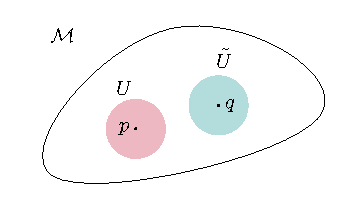
\includegraphics[width=0.4\linewidth]{figures/tikz/hausdorff.pdf}
\caption{Hausdorff'sche Eigenschaft}
\label{img:hausdorff}
\end{figure} 	
	\item[ii)] \textbf{2. Abzählbarkeitsaxiom}  \\
	$\mathcal{M}$ hat eine abzählbare Basis der Topologie, das heißt es existiert eine abzählbare Menge $\{U_1, \dots, U_k, \dots\}$ 
	offener Teilmengen oder abzählbar viele offene Mengen $U_1, \dots, U_k, \dots$ mit $U_i \in \mathcal{O}$, 
	sodass $\forall p \in \mathcal{M}$ und alle Umgebungen $U$ von $p$ gibt es ein $K$ sodass $p \in U_k \subseteq U$.
	\item [iii)] $\mathcal{M}$ ist homöomorph zu $\mathbb{R}^n$, das heißt $\forall p \in \mathcal{M}$ existiert eine Umgebung $U$ von $p$ und ein \bfseries Homöomorphismus \normalfont $X: U \rightarrow V \subseteq \mathbb{R}^n$ (offen).
\end{enumerate} 
\end{defs}
\begin{minipage}[H]{.8\textwidth}
\begin{defs}[Karte, Atlas]
	Das Paar $(X, U)$ heißt \textbf{Karte} von $\mathcal{M}$ um $p$. \\
	Eine Menge $\mathcal{A} = \{(x_{\alpha},U_{\alpha})_{\alpha \in \mathcal{A}}\}$ von Karten heißt \textbf{Atlas} von $\mathcal{M}$, falls \\
	\begin{align}
	\bigcup\limits_{\alpha \in \mathcal{A}} U_\alpha = \mathcal{M}
	\end{align}
\end{defs}
\end{minipage}
\hspace{1cm}
\begin{minipage}[H]{.2\textwidth}
\vspace{-0.5cm}
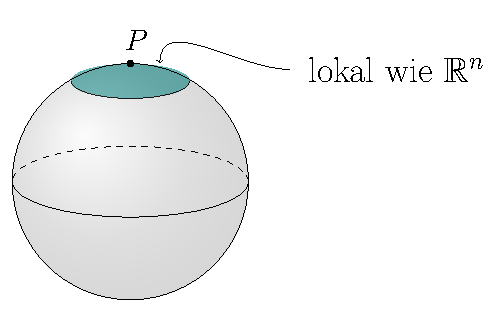
\includegraphics[scale=0.5]{figures/tikz/sphere_local_rn}
\end{minipage}


Topologische Mannigfaltigkeiten sind die Grundbausteine. Nun wollen wir auf diesen Mannigfaltigkeiten Geometrie betreiben. Dafür benötigen wir mehr Struktur. Wir wollen die differenzierbare Struktur des $\mathbb{R}^n$ auf unseren Mannigfaltigkeiten "holen".

\begin{defs}[Kartenwechsel]
Seien $x_{\alpha}$ und $x_{\beta}$ zwei Karten, dann ist der Kartenwechsel wie folgt definiert: \\
\begin{align}
x_{\alpha}\circ x_{\beta}^{-1}: x_{\beta}(U_{\alpha}\cap U_{\beta}) \rightarrow x_{\alpha}(U_{\alpha}\cap U_{\beta}) \subseteq \mathbb{R}^n
\end{align}
Dies ist ein Homöomorphismus.

\begin{figure}[H]
\centering
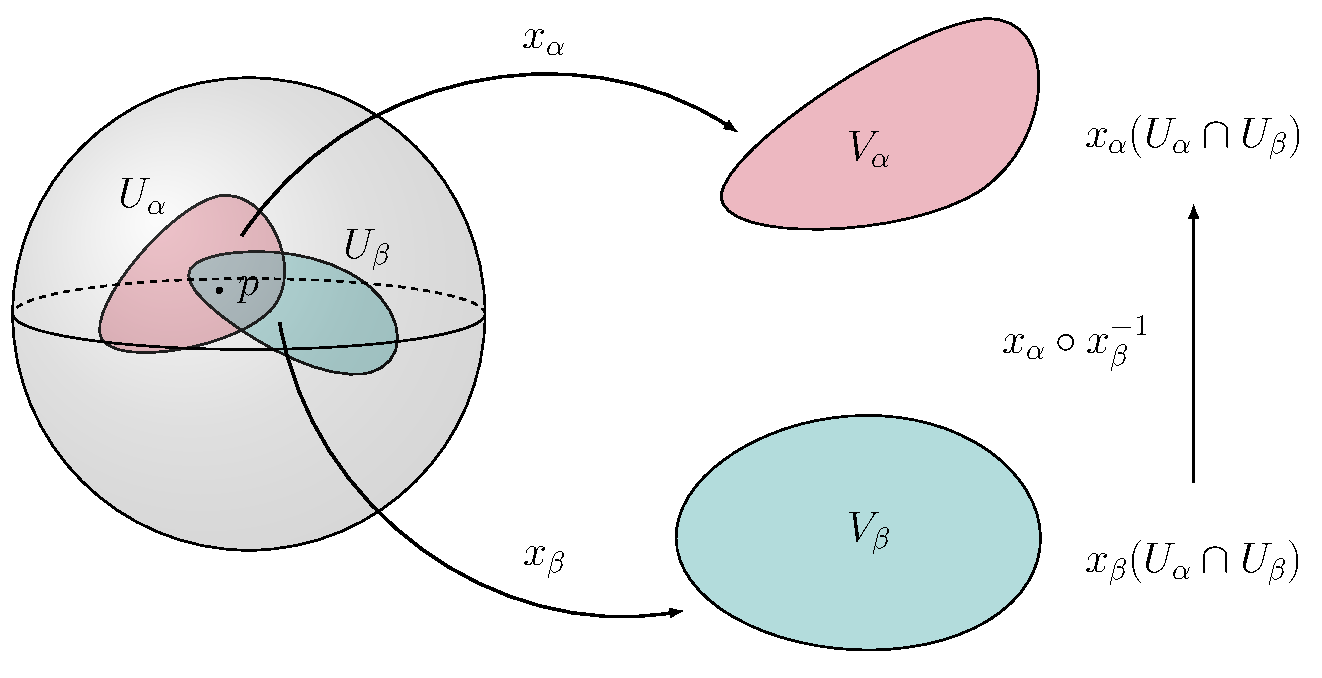
\includegraphics[width=1.0\linewidth]{figures/tikz/map_change.pdf}
\caption{Kartenwechsel}
\label{img:kartenwechsel}
\end{figure} 

\end{defs}
Nun wollen wir, dass $x_{\alpha}\circ x_{\beta}^{-1}$ Diffeomorphismen sind.
\begin{defs}
Sei $ \mathcal{M}$ eine topologische Mannigfaltigkeit.
\begin{enumerate}
	\item[a)] Ein Atlas $\mathcal{A} = \{(x_{\alpha},U_{\alpha})\}$ auf $\mathcal{M}$ heißt $C^{\infty}$-Atlas, falls alle Kartenwechsel $x_{\alpha}\circ x_{\beta}^{-1}$ mit $\alpha, \beta \in A \ C^{\infty}$-Diffeomorphismen sind.
	\item[b)] Sei $\mathcal{A}$ ein $C^{\infty}$-Atlas von $\mathcal{M}$. \\
	Eine Karte $(x,U)$ ist verträglich mit $\mathcal{A}$, falls $x \circ x_\alpha^{-1}$ ein $C^{\infty}$-Diffeomorphismus ist.
\end{enumerate}
\end{defs}
Gegeben ein $C^{\infty}$-Atlas, so kann man diesen zu einem \textit{maximalen} $C^{\infty}$-Atlas vervollständigen. Maximal bedeutet hierbei, dass der Atlas nicht strikt in einem anderen enthalten ist.


	% !TeX root = ..//diffgeo_main.tex
\begin{defs}[Differenzierbare Mannigfaltigkeit]
Eine \textit{differenzierbare Struktur} auf einer topologischen Mannigfaltigkeit $\mfk$ ist ein \textit{maximaler $C^\infty$-Atlas}. Eine \textit{differenzierbare Mannigfaltigkeit} ist eine topologische Mannigfaltigkeit mit einer differenzierbaren Struktur.
\end{defs}

\begin{bem}
Man kann auch eine topologische Mannigfaltigkeit definieren, ohne das 2. Abzählbarkeitsaxiom zu fordern.
\begin{description}
\item[Aber:] Dann bekommt man Mannigfaltigen mit ganz anderen Eigenschaften als diejenigen, die wir betrachten wollen.
\item[Wichtig:] Hausdorffsch + 2. Abzählbarkeitsaxiom $\Rightarrow$ parakompakt, d. h. jede offene Überdeckung hat eine lokal endliche Verfeinerung.
\end{description}
$(V_j)$ heißt Verfeinerung von $(U_i)$, falls $\forall V_j \exists U_i$ mit $V_j \subseteq U_i$\\
Lokal endlich: $\forall p \in X\ \exists$ Umgebung $U$, die nur endlich viele $V_j$ trifft\\
Parakompakt $\Rightarrow \exists$ Partition der Eins f mit 
\begin{align*}
f_i: V_i \subseteq X \rightarrow [0, 1],\ \sum_{i \in I} f_i (x) = 1
\end{align*} 
\end{bem}

\begin{bsp}
Metrische Räume sind parakompakt.
\end{bsp}

\begin{bsp}[differenzierbare Mannigfaltigkeiten]
\begin{enumerate}
\item$\mathbb{R}^n$ mit Atlas $\mathcal{A} = \{(\operatorname{id}, \R^n)\}$
\item$V$ Vektorraum, $B$ Basis mit $B = \{v_1, \cdots, v_n\}$, Atlas $\mathcal{A} = \set{(\chi_B, V)}$
\begin{align*}
& \chi_B: V \rightarrow \R^n\\
& v = \sum^n_{i=1} a_i v_i \mapsto \sum_{i=1}^n a_i e_i
\end{align*}
wobei $(e_1, \cdots, e_n)$ die Standardbasis ist.
\item$\mfk \subseteq \R^n,\ (\chi_U, U)$ mit $\chi_U = \operatorname{id}\vert_U,\ V \subseteq \mfk^n,\ \mfk$ differenzierbare Mannigfaltigkeit, $\mathcal{A} = \set{(\chi_U, U)}$ Atlas von $\mfk$\\
$\mathcal{A}_V = \set{(\chi_V, U_V}$ wobei $(\chi_V, U_V) = (\chi_{U\cap V}, U\cap V)$
\item$\mfk_1 = S^1,\ M_2 = \R,\ M_1\times \mfk_2 =$ "unendlicher Zylinder"

\hspace{.06\textwidth}
\begin{minipage}[H]{0.8\textwidth}
Seien $\mfk_1^{n_1}, \mfk_1^{n_2}$ differenzierbare Mannigfaltigkeiten, so ist $\mfk_1\times \mfk_2$ ebenfalls eine \difM \ der Dimension $n_1 + n_2$.\\
Atlas $\mathcal{A} = \set{(x\times y, U\times V)}$, wobei 
\begin{align*}
(x, U) &= \text{Karte von } \mfk_1\\
(y, V) &= \text{Karte von } \mfk_2
\end{align*}
$(x\times y)(p_1, p_2) = (x(p_1), y(p_2))$
\end{minipage}
\hspace{1cm}
\begin{minipage}[H]{.2\textwidth}
\vspace{-1.5cm}
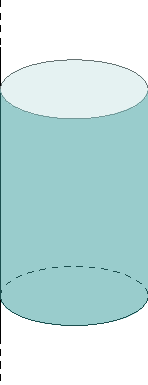
\includegraphics[scale=0.5]{figures/tikz/cylinder.pdf}
\end{minipage}

\item $S_R^n = \{ (x_0, \dots, x_n) \in \R^{n+1} \vert \sum_{i=0}^n x_i^2 = R^2 \} \subset \R^{n+1}$

\begin{itemize}
\item Teilraumtopologie: $U \subset S^n_R$ offen $\Leftrightarrow \exists U' \subset \R^{n+1}$ offen mit $U = U' \cap S^n_R$
\item Atlas: Wir brauchen zwei Karten. 
Einmal für den Nord- und einmal für den Südpol (haben unterschiedliche Orientierung).  \\
Nordpol ($N$):
\begin{align}
f_N : S^n_R \backslash \{ N \} \to \rn \\
f_N (x_0, \dots , x_n) = \frac{R}{R- x_0} (x_1, \dots, x_n) 
\end{align}
Analog für den Südpol (S):
\begin{align}
f_S : \mfk_s \to \rn
\end{align}
\end{itemize}
$\to$ Zwei Karten $f_N$ und $f_S$ ("Stereographische Projektionen").
\begin{figure}[H]
\centering
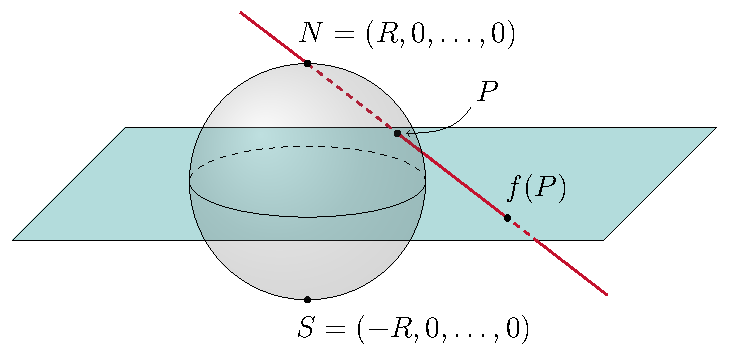
\includegraphics[scale=0.8]{figures/tikz/stereographic_projection.pdf}
\end{figure}
\end{enumerate}
\end{bsp}

\begin{bem}
$N$ mit der Teilraumtopologie und dem Atlas $\mathcal{A}_N = \set{(\chi\vert_U, U\cap N)}$ ist eine \difM.
\end{bem}

\section{Differenzierbare Abbildungen}
\begin{defs}[Differenzierbare Abbildungen]
Seien $\mfk$, $\mfka$ differenzierbare Mannigfaltigkeiten. 
Eine Abbildung $f: \mfk \to \mfka$ heißt differenzierbar, falls $\forall p \in \mfk$ Karten $(x, U)$ von $\mfk$ um $p$ (Karten $(y, V)$ von $\mfka$ um $f(p)$)
\end{defs}
Es gilt: $y \circ f \circ x^{-1}: x(U \cap f^{-1} (U')) \to y(f(U) \cap U')$ ist $\cinf$-differenzierbar.
Wir bezeichnen die Menge aller differenzierbaren Abbildungen durch $\cinf(\mfk, \mfka)$; $\mathcal{F}(\mfk) = \cinf(\mfk, \R)$.

\begin{defs}[Diffeomorphismus]
Eine differenzierbare Abbildung $f: \mfk \to \mfka$ heißt Diffeomorphismus, falls $f$ eine Bijektion und $f^{-1}$ differenzierbar ist. \\
Die Menge aller Diffeomorphismes $f: \mfk \to \mfka$ bezeichnen wir mit $\diff(\mfk, \mfka)$
($\diff(\mfk) \equiv \diff(\mfk, \mfka)$).
Diese bilden eine Gruppe (Diffeomorphismengruppe).
\end{defs}


\section{Untermannigfaltigkeiten}

\begin{defs}[Untermannigfaltigkeiten]
Sei $\mfk$ eine differenzierbare Mannigfaltigkeit. 
Eine Teilmenge $\mfka \subseteq \mfk$ heißt Untermannigfaltigkeit falls:
$\forall p \in \mfka \exists$ Karte $(x, U)$ von $\mfk$ um p $x: \mfk \to V' \times V''$ mit $x(\mfk \cap \mfka) = V' \times \{z_0 \}$
für ein $z_0 \in V''$
\end{defs}


\begin{bem}
$\mfka$ mit der Teilraumtopologie und dem Atlas $\atlas_\mfka = \{ (x_U, U \cap \mfka ) \}$ ist eine differenzierbare Mannigfaltigkeit.
\end{bem}

\begin{defs}[Einbettung]
Seien $\mfk$, $\mfka$ differenzierbare Mannigfaltigkeiten. 
Eine Einbettung ist eine differenzierbare Abbildung
\begin{align}
f: \mfk \to \mfka 
\end{align}
Sodass
\begin{itemize}
\item $f(\mfka) \cap \mfk$ eine Umkehrfunktion.
\item $f: \mfka \to f(\mfka)$ Diffeomorphismus.
\end{itemize}
\end{defs}


\section{Tangentialraum} 

%\missingfigure{Tangentialräume}

\begin{defs}
\begin{enumerate}
\item Ein Tangentialvektor an $\mfk$ im Punkt $p \in \mfk$ ist eine $\R$-lineare Abbildung
\begin{align*}
v: \mathcal{F}(\mfk) \rightarrow \R
\end{align*}
mit $v(fg) = v(f)g(p) + f(p)v(g)$.
\item Die Menge aller Tangentialvektoren an $\mfk$ in $p$ heißt \textit{Tangentialraum} von $\mfk$ in $p$: $T_p \mfk$\\
$T_p \mfk$ ist ein Vektorraum.
\end{enumerate}

\begin{figure}[H]
\centering
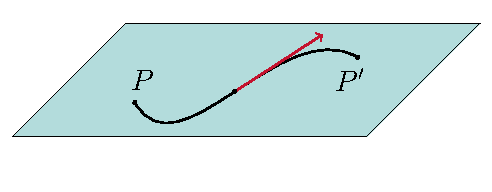
\includegraphics[scale=1]{figures/tikz/tangentline.pdf}
\end{figure}
\end{defs}

	% !TeX root = ..//diffgeo_main.tex
\begin{hlem}[Existenz einer Glockenfunktion]
Sei $U \subseteq \mfk$ offen, $p \in U$. Dann $\exists \varphi \in \mathcal{F}(\mfk)$, s. d. 
\begin{enumerate}\label{Glockenfunktion}
\item$\operatorname{supp}\varphi\subseteq U$
\item$\varphi=1$ auf einer Umgebung $U' \subset U$ von $p$ ist
\end{enumerate}
\end{hlem}

\begin{figure}[H]
\centering 
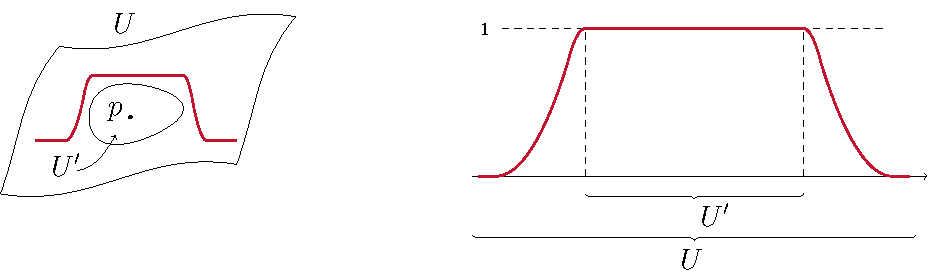
\includegraphics[scale=0.8]{figures/tikz/bump_function.pdf}
\caption{Visualisierung des Hilfslemmas  (\ref{Glockenfunktion}) \  ("bump function") }
\end{figure}

\begin{bew}
Sei $(x, U)$ eine Karte um $p$, $\epsilon > 0$, s. d. $B_{2\varepsilon}(x(p))\subset V\subset \R^n$ und wähle $\psi:\R^n\rightarrow\R$ mit 
\begin{align*}
\left.
\begin{array}{r}
\operatorname{supp}(\psi)\subset B_{2\epsilon}(x(p))\\
\varphi = 1 \text{ auf } B_\epsilon
\end{array}
\right\} \text{ Resultat aus Analysis}\\
\end{align*}

Setze $\varphi(q) = \left\{
\begin{array}{l}
\psi(x(q))\text{ für }q\in U\\
0 \text{ sonst}
\end{array}
\right.$
\end{bew}

\begin{satz}[Eigenschaften des Tangentialraums]
Für $v\in T_p \mfk$ gilt:
\begin{enumerate}
\item$v(\text{konstante Funktion}) = 0$
\item Falls $f = g$ in einer Umgebung von $p$, so gilt $v(f) = v(g)$
\end{enumerate}
"Lokalisierung von Tangentialvektoren"
\end{satz}

\begin{bew}[zu 2]
Wähle $\varphi$ wie im Hilfslemma, wobei $U$so gewählt ist, dass $\varphi f = \varphi g$ auf $U$ ist. Nun gilt:
\begin{align*}
v(\varphi f) &= v(\varphi)f(p) + \varphi(p)v(f)\\
&= v(\varphi)f(p) + v(f)\\
v(\varphi g) &= v(\varphi)g(p) + v(g)
\end{align*}
Dann folgt $v(\varphi f) = v(\varphi g) \Leftrightarrow v(f) = v(g)$.
\end{bew}

\begin{bew}[zu 1]
	$v(\lambda f) = \lambda v(f),\ \lambda \in \R,\ f\in \mathcal{F}(\R)$\\
	\textit{zz:} $v(\lambda) = 0$. 
	Aufgrund von $v(\lambda) = \lambda v(1)$ genügt es zu zeigen, dass $v(1) = 0$. Dies folgt aus der Produktregel
	\begin{align*}
	v(1) = v(1*1) = 1v(1) + v(1)1 = 2v(1) \Rightarrow v(1) = 0
	\end{align*}
\end{bew}


	Jede Karte liefert eine spezielle Basis von $T_p \mfk$.

\begin{defs}
Sei $(x, U)$ eine Karte von $\mfk$ um $p$. 
Definiere Tangentialvektoren $\pdv{x_i} \eval_{p} $ ($i = 1, \dots, m$) wie folgt:
\begin{align}
\pdv{x_i}\eval_{p} (f) := \partial_i (f \circ x^{-1}) \eval_{x(p)}
\end{align}
Hierbei bedeutet $\partial_i$ die $i$-te partielle Ableitung.
\end{defs}

\begin{satz}
\label{satz:BasisTPM}
Die Tangentialvektoren $(\pdv{x_1}\eval_{p}, \dots, \pdv{x_m}\eval_{p})$ bilden eine Basis des $\tspace{p}$.
Jeder Tangentialvektor lässt sich schreiben als
\begin{align}
v = \sum_{i=1}^{m} v(x_i) \pdv{x_i}\eval_{p} = \sum_{i=1}^{m} \xi \pdv{x_i}\eval_{p}.
\end{align}
\end{satz}
\begin{bew}[Satz \ref{satz:BasisTPM} Teil 1]
Es gilt die lineare Unabhängigkeit:
\begin{align}
\pdv{x_1}\eval_{p} (x^j) = \delta_{i j}
\end{align}
Jetzt muss noch gezeigt werden, dass $(\pdv{x_1}\eval_{p}, \dots, \pdv{x_m}\eval_{p})$ ein Erzeugendensystem für $\tspace{p}$ ist.
 Dafür benötigen wir allerdings zunächst ein Hilfslemma.
\end{bew}

\begin{hlem}
\label{lem:DarstellungBasisTPM}
Sei $f: U \subset \mfk \to \R$ eine glatte Funktion.
Dann existiert eine Umgebung $U' \subset U$ von $p$ ($p \in U'$) und eine glatte Funktion
$f_i: U' \to \R$, so dass
\begin{align}
f = f(p) + \sum_{i=1}^{m} ( x_i  - x_i(p)) f_i.
\end{align}
Wobei $f_i (p) = \pdv{x_i}\eval_{p} (f)$.
\end{hlem}

\begin{bew} \leavevmode

\begin{figure}[H]
\centering
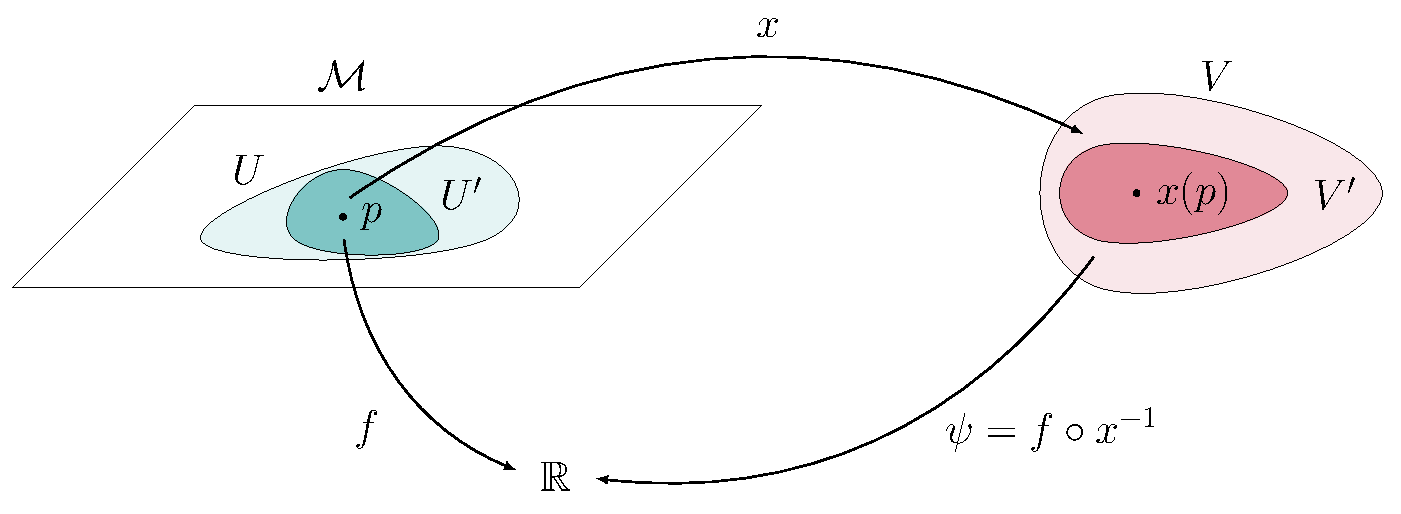
\includegraphics[width=1\linewidth]{figures/tikz/lemma_tangentialvectors.pdf}
\label{img:lemmaDarstellungBasisTPM}
\end{figure}

Nach der Abbildung gilt:
\begin{align}
\psi(U) - \psi(U_0) = \int^1_0 \dv{t} \psi(t U + (1- t) U_0) \dd t
\end{align}
Hierbei ist $U=x(q)$ mit $q \in \mfk$ und $U_0 = x(p)$.
\begin{align}
\psi(U) - \psi(U_0) = \sum_i (U^i- U^i_0) \int^1_0 \underbrace{\dv{\psi}{U'} (t U + (1 - t) U_0) \dd t}_{:= \psi_i (U)}
\end{align}
Setze $f_i = \psi_i \circ x : U \subset \mfk \to \R$.
$f_i$ ist glatt und es gelten folgende Eigenschaften nach Definition:
\begin{itemize}
\item $\psi(U)- \psi(U_0) = \psi(x(q)) - \psi(x(p)) = f(q)- f(p)$
\item $U^i = x^i (q)$
\item $U_0^i = x^i(p)$
\item $\psi_i (U) = \psi_i (x(1)) = f_i(q)$
\end{itemize}
Diese Eigenschaften können wir nun wie folgt verwenden:
\begin{align}
f(q)- f(p) = \sum_{i=1}^n (x_i (q) - x_i (p)) f_i(q)
\end{align}

\begin{align}
\pdv{x_i}\eval_{p} (f) &= \partial_i \underbrace{(f \circ x^{-1})}_{\psi} \big \vert_{x(p)} \\
&= \partial_i \psi \eval_{x(p)}\\
&= \psi_i (x(p)) = f_i (p)
\end{align}
Da $\psi(U) = \psi(U_0) + \sum_i (U^i - U^i_0)\psi_i(U)$
\begin{align}
\Rightarrow \pdv{U_i} \psi \eval_{x(p)} = \psi_i(U) \eval_x(p) = \psi(x(p))
\end{align}
Und somit gilt schließlich $f_i (p) = \pdv{U_i} \eval_p (f)$.
\end{bew}

Nun können wir unseren Beweis fortführen.

\begin{bew}[Satz \ref{satz:BasisTPM} Teil 2] \leavevmode
\begin{align}
v(f) &= v(f(p) + \sum_i (x_i - x_i(p)) f_i) \\
&= v(f(p)) + \sum_i v(x_i - x_i (p) f_i)
\end{align}
Benutze Produktregel
\begin{align}
v(f) &= \sum_i (\underbrace{(x_i (p) - x_i (p)) v(f_i)}_{=0} + \underbrace{v(x_i - x_i (p))}_{=v(x_i)} f_i) \\
&= \sum_i v(x_i) f_i \\
&= \sum_i v(x_i) \pdv{x_i} \eval_p f 
\end{align}
\end{bew}

\begin{satz}[Transformationsregel]
Seien $(x, U)$ und $(\tilde{x}, \tilde{U})$ zwei Karten um $p \in \mfk$.
\begin{figure}[H]
\centering
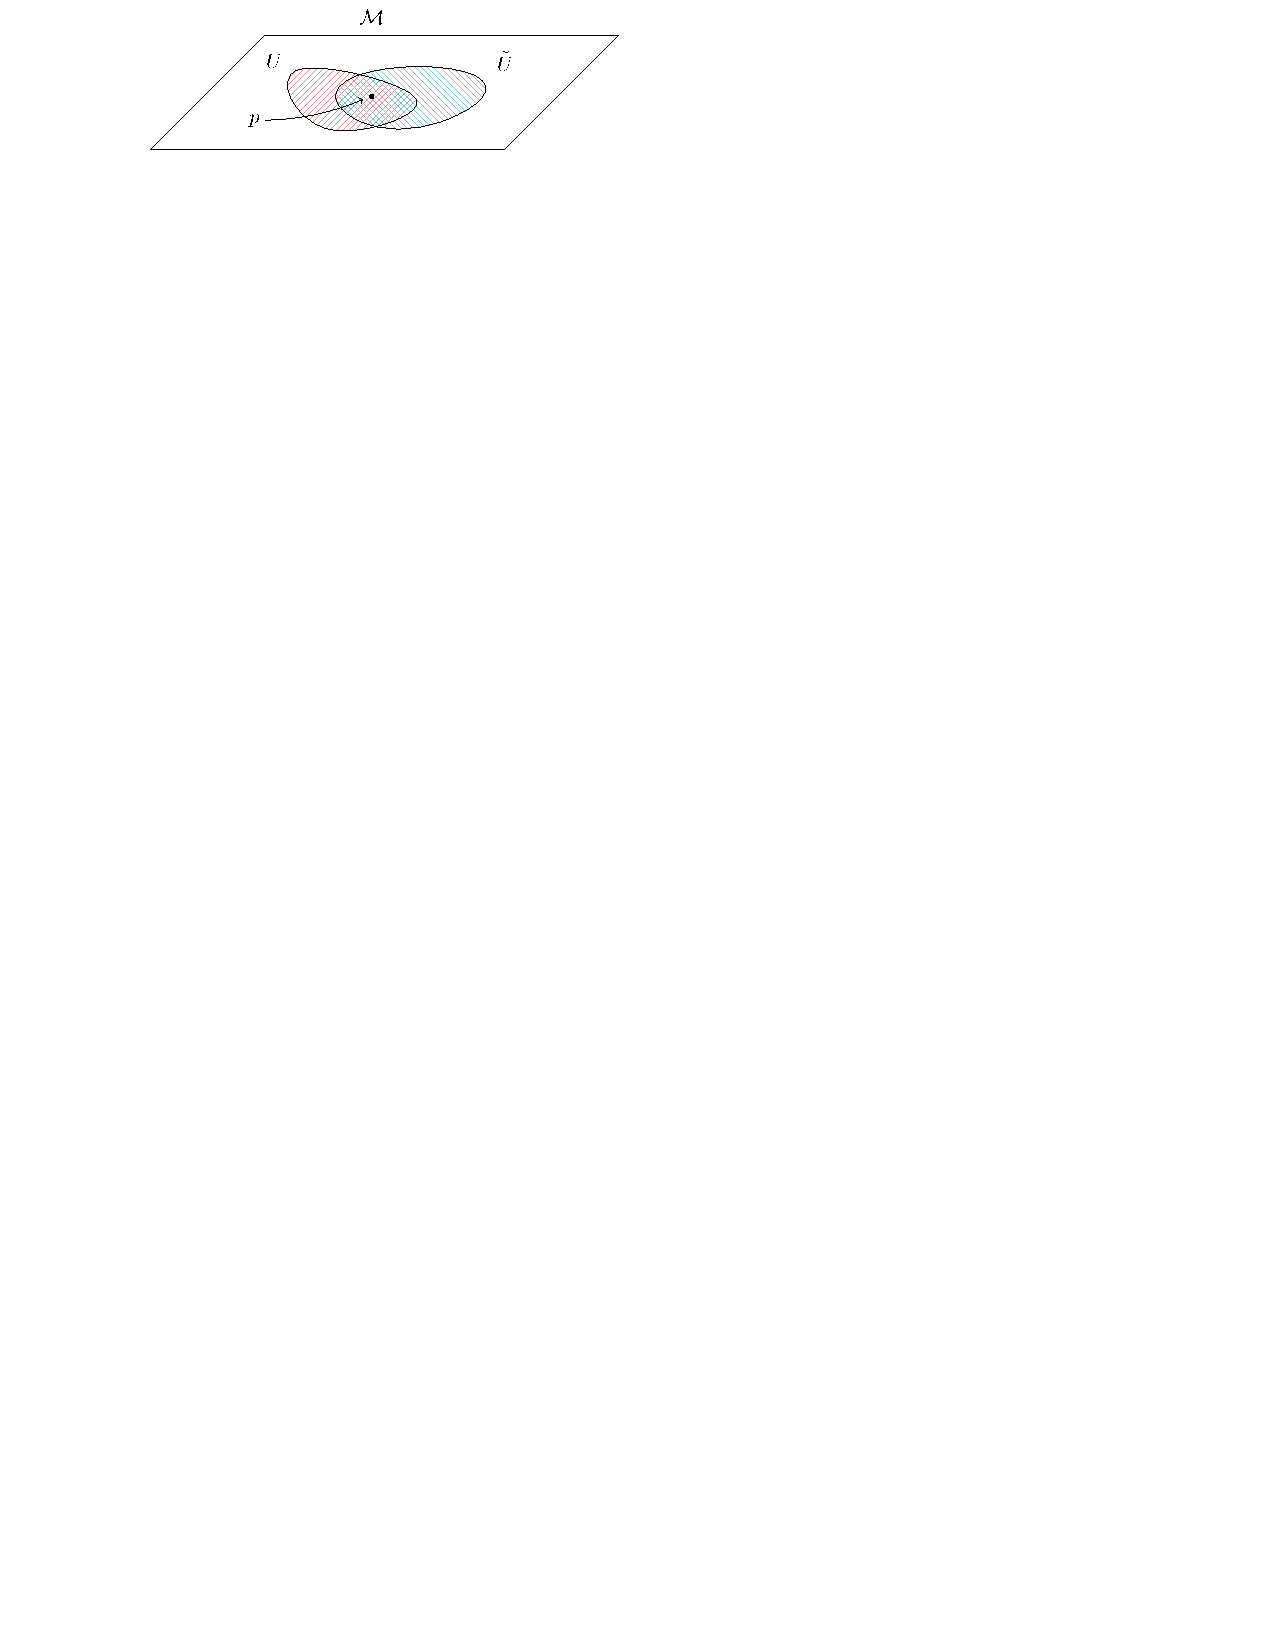
\includegraphics[scale=1.0]{figures/tikz/transformationlaw.pdf}
\label{img:transformationsregel}
\end{figure}  
Dann gilt:
\begin{align}
\pdv{\tilde{x}_i} \eval_p  = \sum_j \underbrace{\pdv{\tilde{x}_i} \eval_p  (x_j)}_{\in \R} \pdv{x_j} \eval_p 
\end{align}
(In der lineare Algebra hatten Transformation die ähnliche Gestalt: $\tilde{v}_i = \sum_j a_{i j } v_j$)
\end{satz}
\begin{defs}[Differential, Ableitung]
Seien $\mfk$ und $\mfka$ differenzierbare Mannigfaltigkeiten und $f: \mfk \to \mfka$ glatt.
Das \textbf{Differential (Ableitung)} von $f$ in $p$ ist die lineare Abbildung:
\begin{align}
\dd f \eval_p : \tspace{p} &\to T_{f(p)}\mfka \\
v &\mapsto \dd f \eval_p (v),
\end{align}
welche definiert ist durch:
\begin{align}
\underbrace{\dd f \eval_p (v)}_{T_{f(p)}\mfka} \underbrace{(\phi)}_{\in \mathcal{F}(\mfk)} = \underbrace{v(\phi \circ f)}_{\in \mathcal{F}(\mfka)}, \quad \forall p \in \mathcal{F}(\mfka)
\end{align}
\end{defs}
Fakt: $\dd f \eval_p$ ist linear.
\begin{satz}[Kettenregel]
\label{satz:Kettenregel}
Seien $f: \mfk \to \mfka$ und $g: \mfka \to \mathcal{P}$ glatte Abbildungen.
Dann gilt:
\begin{align}
\dd (g \circ f) \eval_p = \dd g \eval_{f(p)} \circ \dd f \eval_p
\end{align}
\begin{figure}[H]
\centering
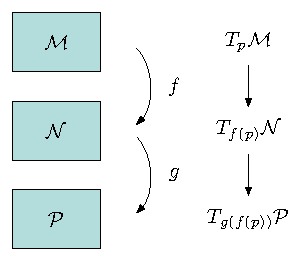
\includegraphics[width=0.45\linewidth]{figures/tikz/chain_rule.pdf}
\label{img:kettenregel}
\end{figure} 
\end{satz}

\begin{bew}[Satz \ref{satz:Kettenregel}] \leavevmode
\begin{align}
\dd (g \circ f) \eval_{p} (v (\phi)) &= v(\phi \circ g \circ f) \\
&= \dd f \eval_p (v)(\phi \circ g) \\
&= \dd g \eval_{f(\phi)} \circ \dd f \eval_p (v) (\phi)
\end{align}
\end{bew}

\begin{satz}
Sei $f: \mfk \to \mfka$ glatt und sei $(x, U)$ eine Karte von $\mfk$ um $p$ und $(y, V)$ eine Karte von $\mfka$ um $p$.
Setze $f_j = y_j \circ f$ mit $f_j : \mfk \to \R$, dann gilt:
\begin{align}
\underbrace{\dd f \eval_p ( \pdv{x_i} \eval_p)}_{\in T_{f(p)}\mfk} = \sum_j \underbrace{\pdv{x_i}\eval_p (f_j)}_{\in \R} \underbrace{\pdv{y_j} \eval_{f(p)}}_{\in T_{f(p)}\mfka}
\end{align}
\end{satz}

\begin{defs}[regulärer Wert/Punkt, Submersion, Immersion] 
Sei $f: \mfk \to \mfka$ glatt und es gelte $\dim\mfk=m$, $\dim{\mfka} = n$.
\begin{enumerate}
\item $\rang f$ in $p$ ist $\rang \dd f \big \vert_p $.
\item $p\in\mfk$ heißt regulärer Punkt ($\in\mfk$)  $\Leftrightarrow \rang\dd f \eval_p=\dim\mfka$.
\item $q\in\mfka$ heißt reguläreer Wert ($\in\mfka$) $\Leftrightarrow \forall p \in f	^{-1}(q)$ sind reguläre Punkte.
\item $f$ heißt Submersion $\Leftrightarrow$ $f$ surjektiv und alle $p\in\mfk$ reguläre Punkte sind.
\item $f$ heißt Immersion $\Leftrightarrow$ $\dd f \eval_p$ injektiv für alle $p \in \mfk$
\end{enumerate}
\end{defs}

\begin{satz}[Umkehrsatz]
\label{satz:Umkehrsatz}
Sei $f: \mfk \to \mfka$ glatt. 
Sei $\dd f \eval_p : \tspace{p} \to T_{f(p)}\mfka$ ein Isomorphismus,
dann existiert eine Umgebung $U$ um $p$ und eine Umgebung $U'$ um $f(p)$, so dass
\begin{align}
f\eval_U : U \to U'
\end{align}
ein Diffeomorphismus ist.
\begin{figure}[H]
\centering
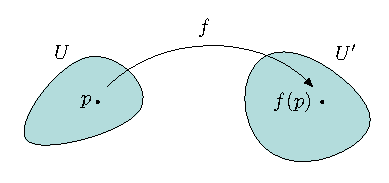
\includegraphics[width=0.5\linewidth]{figures/tikz/inverse_function_theorem.pdf}
\label{img:umkehrsatz}
\end{figure} 
\end{satz}

\begin{bew}[Satz \ref{satz:Umkehrsatz}] \leavevmode
Nutze Karten um dies auf den euklidischen Fall zu führen.

\begin{align}
\begin{xy}
  \xymatrix@=0.25\linewidth{
      \mfk \ar[r]^f \ar[d]_x    &   \mfka \ar[d]^y \\
      V\subseteq \R^m \ar[r]_\phi             &   V\subseteq \R^m    
  }
\end{xy}
\end{align}

Seien $(x, U)$ und $(y, U')$ Karten von $\mfk$ und $\mfka$ um $p$ und $f(p)$.
Ohne Beschränkung der Allgemeinheit gilt: $f(U) \subset U'$.
Dann ist $\phi$ eine glatte Abbildung deren Differential $\dd \phi \eval_{x(p)}$ invertierbar ist.
Umkehrsatz im $\rn$ auf $\phi$ anwenden:
Es existieren Umgebungen $\hat{V}$ von $x(p)$ und $\hat{V}'$ von $y(f(p)) = \phi(x(p))$, so dass
$\hat{\phi}\eval_{\hat{V}}$ ein Diffeomorphismus ist.
Dann ist
\begin{align}
f\eval_{x^{-1}(\hat{V})}: x^{-1}(\hat{V}) \to y^{-1}(\hat{V}')
\end{align}
ein Diffeomorphismus.
\begin{align}
\phi = y \circ f \circ x^{-1} \Rightarrow f = y^{-1} \circ \phi \circ x
\end{align}
\end{bew}


\begin{satz}[Satz über implizite Funtionen]
\label{satz:Satz über implizite Funtionen}
\end{satz}
Sei $f: \mfk \to \mfka$ glatt und es gelte $\dim\mfk=m$, $\dim{\mfka} = n$.
\begin{enumerate}
\item Sei $\rang_p f = r$. 
Dann existiert zu jeder Karte  $(y, U')$ um $f(p)$ eine Karte $(x, U)$ um $p$, so dass
\begin{align}
y \circ f \circ x^{-1}(U_1, \dots, U_m) = (U_1, \dots, U_r, \phi_{r+1}(U), \dots, \phi_n(U)).
\end{align}
Falls $y(f(p))=0$, so kann man $x$ so wählen, dass $x(p)=0$ und $\phi_j (0) = 0$ ($\forall j > r$).

\item Sei $\rang f = r$ auf einer Umgebung von $p$.
Dann gibt es Karten $(x, U)$, $(y, U')$, so dass 
\begin{align}
y\circ f \circ x^{-1} (U_1, \dots, U_m).
\end{align}

\end{enumerate}
\begin{bew}[Satz \ref{satz:Satz über implizite Funtionen} Teil 1]
Wähle Karten und modifiziere diese geschickt.
Sei $(y, U')$ eine Karte von $\mfka$ um $f(p)$.
Sei $(\hat{x}, U)$ eine Karte von $\mfk$ um $p$ mit $\hat{x}(p) = 0$.
Setze 
\begin{align}
\hat{A} = (\hat{A})_{i j} = (\partial_i \hat{\phi}_j),
\end{align}
mit $\phi \circ y \circ f \circ x^{-1}$.
Da $\rang_p f = r$, können wir ohne Beschränkung der Allgemeinheit annehmen, dass
\begin{align}
\det \tilde{A} \neq 0.
\end{align}
Wobei hier nun $\tilde{A} = (\hat{A}_{i j})_{1 \leq i \leq r}$.
Setze 
\begin{align}
x_i = \left\{
\begin{array}{ll}
y_i \circ f & \quad 1 \leq i \leq r \\
\hat{x}_i & \textrm{falls} \ r+1 \leq i \leq n \\
\end{array}
\right. 
\end{align}
Dann gilt $x(p)=0$ und 
\begin{align}
\partial_i (x_j \circ \hat{x}^{-1})(0) = 
\left(\begin{matrix}
\partial_i \hat{\phi}_j (0) & \star \\ 
0 & \mathds{1}
\end{matrix} \right) .
\end{align}
Daraus folgt, dass $\rang x = m = \dim \mfk$ im Punkt $p$.
Mit Hilfe des Umkehrsatzes folgt, dass $x$ ein lokaler Diffeomorphismus ist 
und eine Umgebung $U$ um den Punkt $p$ existiert und eine Umbegungen $V$ von $0$ in $\rn$, 
sodass $x: \mfk \to V$ eine Karte ist und
\begin{align}
\phi (U_1, \dots, U_m) &= y \circ f \circ x^{-1}(U_1, \dots, U_m) \\
&= (U_1, \dots, U_r, \phi_{r+1}(U), \dots, \phi_m (U)).
\end{align}
Wobei $\phi_k$ glatt auf $U'$ sint mit $\phi_i(0)=0$. 
Betrachte die Jacobi-Matrix:
\begin{align}
A_{i j} = (\partial _i \phi_j )_{i j} = \begin{pmatrix}
\mathds{1} & 0 \\ 
\star & \partial_i \phi_i
\end{pmatrix} 
\end{align}
Da $\rang \phi = r$ in einer Umgebung von $U=0$ hat folgt:
\begin{align}
\partial_i \phi_j \quad \forall i, j > r.
\end{align}
\end{bew}

\begin{kor}
Sei $f: \mfk \to \mfka$ mit $\dim \mfk = m$ und $\dim \mfka = n$ glatt, dann gilt:
\begin{enumerate}
\item Sei $q \in \mfka$ ein regulärer Wert, so ist 
\begin{align}
\mathcal{H} = f^{-1}(q) = \{ p \in \mfk (f(p))=q \}
\end{align}
eine Untermannigfaltigkeit der Dimension $m-n$.
\item Sei $f$ linear in einer Umgebung von $\mathcal{H} = f^{-1}(q)$ vom $\rang$ $r$, so ist $\mathcal{H}$ eine Untermannigfaltigkeit der Dimension $m-r$.
Der Tangentialraum $T_p \mathcal{H}$ ist isomorph zu
\begin{align}
\ker \dd f \eval_p \subseteq \tspace{p}, \quad \forall p \in \mathcal{H}.
\end{align}
\end{enumerate} 
\end{kor}
	% !TeX root = ..//diffgeo_main.tex
\chapter{Vektorbündel}
\section{Tangentialbündel}
Wir wollen nun alle Tangentialräume einer Mannigfaltigkeit $\mfk$ gemeinsam betrachten.
\begin{align}
T\mfk = \bigsqcup_{p\in \mfk} T_{p}\mfk = \{ (p, V) \vert p \in \mfk, v \in T_{p}\mfk \} 
\end{align}
Dies soll nun die Struktur einer differenzierbaren Mannigfaltigkeit haben. 
Das heißt wir müssen eine Topologie und eine $\cinf$-Struktur auf $T\mfk$ definieren.
\begin{align}
\pi: T\mfk &\to \mfk \\
(p,V) &\mapsto p
\end{align}
Sei $(x, U)$ eine Karte von $\mfk^m$. 
Dann definieren wir eine Karte $(\overline{x}, \overline{U})$ von $T\mfk$ wie folgt:
\begin{align}
&\overline{U} = \pi^{-1}(U) = \bigsqcup_{p\in\mfk} T_{p}\mfk \\
&\overline{x}: \overline{U} \to x(U) \times \R^m \subset \R^{2m} \\
&(p, V) \mapsto (x(p), \xi)
\end{align}
Wobei $\xi = (\xi^1, \dots, \xi^m) \in \R^m$ gegeben ist durch:
\begin{align}
v = \sum_{i=1}^{m} \xi_i \pdv{x_i} \big\vert_p, \quad \forall p \in U.
\end{align}
Wir können aber Kartenwechsel betrachten.\\
Seien $(\overline{x}, \overline{U})$ und $(\overline{y}, \overline{U}')$ zwei Karten. 
Betrachte die Abbildungen:
\begin{align}
\overline{y} \circ \overline{x}^{-1} \circ \underbrace{x (\overline{U} \cap \overline{U}')}_{x(U \cap U') \times \R^m} \to \underbrace{\overline{y}(\overline{U} \cap \overline{U}')}_{y(U \cap U') \times \R^m}
\end{align}
\begin{align}
(x,\xi) \mapsto (y\circ x^{-1}(U), \eta) 
\end{align}
Wobei $\eta = \dd (y \circ x^{-1})\eval_U \xi$.\\
Da $y\circ x^{-1}$ Diffeomorphismus ist, ist $\overline{y} \circ \overline{x}^{-1}$ ein Isomorphimus.
Nun können wir die Topologie auf $T\mfk$ definieren.
$O \subset T\mfk$ offen, falls $\overline{x}(O\cap \overline{U})$ offen in $V \times \R^m$ ist für alle Karten $(x, U) \in \atlas_\mfk$ (bzw $(\overline{x}, \overline{U}) \in \atlas_{T\mfk}$)

\begin{satz}
$T\mfk$ mit dieser Topologie ist eine topologische Mannigfaltigkeit und $\atlas_{T\mfk}$ eine differenzierbare Struktur.
\end{satz}
\section{Vektorbündel}
$T\mfk$ hat die Struktur einer glatten Mannigfaltigkeit.
Allerdings hat es noch mehr, nämlich die eines Vektorbündels, was wir nun definieren.
\begin{defs}[Vektorbündel]
Sei $\mfk$ eine differenzierbare Mannigfaltigkeit.
Ein $\R$-Vektorbündel vom $\rang$ $k$ über $\mfk$ ist eine differenzierbare Mannigfaltigkeit mit einer glatten surjektiven Abbildung:
\begin{align}
\pi: E \to \mfk,
\end{align}
so dass:
\begin{enumerate}
\item $\forall p \in \mfk$ hat $E_p:= \pi^{-1}( \{ p \})$ die Struktur eines $\R$-Vektorraums der Dimension $k$.
$E_p$ heißt Faser von $E$ über $p$.
\item Für alle $p$ in $\mfk$ existiert eine Umgebung $U$ von $p$ in $\mfk$ und ein Diffeomorphismus, für den gilt:
\begin{itemize}
\item $\pi \circ \phi = p r_1$
\item Für alle $q \in U$ ist die Abbildung
\begin{align}
&\phi\eval_q : \{ q \} \times \R^k \to E_q\\
&\{ q, \xi \} \mapsto \phi_q (\xi) := \phi(q, \xi)
\end{align}
$\phi$ heißt lokale Trivialisierung von $E$.
\end{itemize}
\end{enumerate}
\begin{align}
\begin{xy}
\xymatrix@=0.15\linewidth{
      \phi: U \times \R^k \ar[rr] \ar[rd]_{pr_1}  &     &  \pi^{-1}(U) \ar[dl]^{\pi}  \\
                             &  U  &}
\end{xy}
\end{align}
\end{defs}
\begin{bem}
Ein Vektorbündel ist ein Tripel $(E, \pi, \mfk)$ aber wir schreiben oft nur $E$. Hierbei wird $E$ Totalraum und $\mfk$ Basis genannt.
\end{bem}
\begin{figure}[H]
\centering
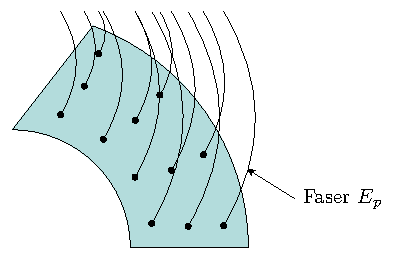
\includegraphics[scale=1.1]{figures/tikz/vectorbundel.pdf}
\caption{Veranschaulichung eines Vektorbündels}
\label{img:tangentialbuendel}
\end{figure}
\begin{bsp} \leavevmode
\begin{enumerate}
\item Triviales Bündel:
\begin{align}
&E = \mfka \times \R^k \to \mfk\\
&(p, \xi) \mapsto p
\end{align}
\item Tangentialbündel 
\begin{align}
&\pi: T\mfk \to \mfk\\
&(p, V) \to V
\end{align}
\begin{figure}[H]
\centering
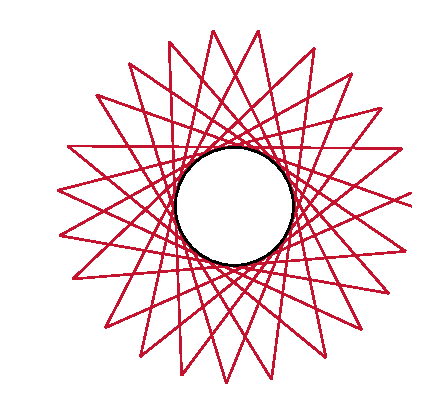
\includegraphics[scale=0.7]{figures/tikz/tangent_bundle.pdf}
\caption{Darstellung des Tangentialbündels eines Kreises}
\label{img:tangent_bundle}
\end{figure}

\item Tautologisches Bündel
\begin{align}
&\mfk = \R \mathbb{P}^n\\
&E = \{ (l, x) \vert l \in \R \mathbb{P}^n, x\in l \subset \R^{n+1} \}\\
&\pi: E \to \mfk = \R \mathbb{P}^n\\
&(l, x) \mapsto l
\end{align}
Behauptung: Dies ist ein Vektorbündel vom $\rang$ $1$.
Vektorraumstruktur auf $E_l$:
\begin{align}
(l, x) + (l, y) &:= (l, x + y)\\
k (l, x) &:= (l, k x)
\end{align}
\end{enumerate}
\end{bsp}
Nun wollen wir uns damit beschäftigen wie wir Vektorbündel konstruieren können.
Angenommen uns wäre das folgende gegeben:
\begin{enumerate}
\item $E_p$ (mit $p\in \mfk$) eine Familie von Vektorräumen der Dimension $k$
\item $(U_\alpha)_{\alpha \in A}$ eine offene Überdeckung von $\mfk$
\item $\forall \alpha \in A$, $p\in U_\alpha$ gibt es den folgenden Isomorphismus:
\begin{align}
\phi_{\alpha, p}: \R^\alpha \to E_p
\end{align}
\end{enumerate}
Setze 
\begin{align}
&E = \bigcup_{p \in \mfk} E_p\\
&\pi : E \to \mfk\\
&(p, V) \mapsto p\\
&\phi_\alpha: U_\alpha \times \R^k \to E \eval_{U_\alpha}\\
&(p, \xi) \mapsto (p, \phi_{\alpha, p}(\xi)).
\end{align}
Nun stellt sich die Frage unter welchen Vorraussetzungen $(E, \pi, \mfk)$ ein Vektorbündel ist.
\begin{lem}
\label{lem:vorraussetzungenvektorbündel}
Sei $\mfk$ eine glatte Mannigfaltigkeit, $E$ eine Menge und die Abbildung $\pi: E\to\mfk$ surjektiv.
Sei $\{ U_\alpha \}$ eine offene Überdeckung von $\mfk$ zusammen mit bijektiven Abbildungen
\begin{align}
\phi^{-1}_{\alpha} = \varphi: \pi^{-1}(U_\alpha) \to U_\alpha \times \R^\alpha,
\end{align}
die $pr_1 \circ \varphi_\alpha = \pi$ erfüllen, so dass wann immer $U_\alpha \cap U_\beta \neq \emptyset$, dann ist 
\begin{align}
\varphi_\alpha \circ \varphi_{\beta}^{-1} \to (U_\alpha \cap U_\beta) \times \R^k,
\end{align}
von der Form:
\begin{align}
\label{eq:konstruktionvektorbündel}
(\varphi_\alpha \circ \varphi_{\beta}^{-1})(p, v) = (p, \tau(p) v)
\end{align}
mit einer glatten Abbildung $\tau: U_\alpha \cap U_\beta \to \mathrm{GL}(k, \R)$.
Dann existiert eine eindeutige Struktur als glattes $k$-dim Vektorbündel über $\mfk$ für die $\varphi^{-1}_{\alpha}$ lokale Trivialisierungen sind.
\end{lem}
\begin{bew}[Lemma \ref{lem:vorraussetzungenvektorbündel}]
Sei  $p\in\mfk$ und setze $E_p := \pi^{-1}(\{ p \})$. 
Falls $p\in U_\alpha$, dann ist 
\begin{align}
\varphi_\alpha \eval_p : E_p \to \{ p \} \times \R^k.
\end{align}
Definiere eine Vektorraumstruktur auf $E_p$ durch die Forderung, dass die Abbildung $\varphi_\alpha \eval_p$ ein Isomorphismus ist.
Durch verkleinern von $U_\alpha$ und hinzunahme von weiteren offenen Mengen kann man annehmen, dass jedes $U_\alpha$ diffeomorph zu $\overline{U}_\alpha \subseteq \R^m$ ist.
Verknüpfung von $\varphi_\alpha$ mit einem solchen Diffeomorphismus liefert eine Bijektion:
\begin{align}
\pi^{-1} (U_\alpha) \to \overline{U}_\alpha \times \R^k .
\end{align}
Diese nutzen wir als Karte für $E$.
Wegen Gleichung \ref{eq:konstruktionvektorbündel} bekommen wir eine glatte Struktur auf $E$.
\end{bew}
Sei $(x, U)$ Karte von $\mfk$, $p\in U$, $v\in T_p \mfk$.
\begin{align}
v = \sum_{i=1}^{m} \xi_i \pdv{x_i}\eval_p
\end{align}
Definiere:
\begin{align}
\varphi: \pi^{-1} (U) &\to U \times \R^m\\
v &\mapsto (p, V)
\end{align}
Dort wo $(x)$ und $(\overline{x})$ überlappen.
\begin{align}
\pdv{x_i} \eval_p &= (\pdv{\overline{x}_j}{x_i})\pdv{\overline{x}_j} \eval\\
v &= \sum_{j=1}^{m} \xi_j \pdv{\overline{x}_j}  \eval_p = \sum_{ji1}^{m} \xi_i \pdv{\overline{x}_i}  \eval_p \\
&= \sum_{i, j}^{m} \xi_i \pdv{\overline{x}_j}{x_i}  \pdv{\overline{x}_j}\eval_p\\
&\Rightarrow \overline{\xi}_j = \sum_i v_i \pdv{\overline{x}_j}{x_i}
\end{align}
\begin{align}
\varphi \circ \varphi^{-1}(x, v) = (x, \overline{v}) = (x, \tau(x) v)
\end{align}
Wobei nun $\tau(x)$ gegeben ist durch $\pdv{\overline{x}_j}{x_i}$.\\
	% !TeX root = ..//diffgeo_main.tex
Im Folgenden werden nun einige Beispiele für Vektorbündel angeben.
\subsection{Direkte Summe (Whitney-Summe)}
Es seien zwei Vektorbündel gegeben:
\begin{align}
\pi : E &\to \mfk \\
\pi ' : E' & \to \mfk '
\end{align}
mit $\rang$ $k$ bzw. $k'$. 
Dann existiert $(U_\alpha)_{\alpha \in A}$ eine offene Überdeckung, sodass für alle $\alpha \in A$ und alle $p \in U_\alpha$ folgendes gilt:
\begin{align}
&\phi_{\alpha, p}: \R^k \to E_p, \quad g_{\alpha, \beta}: U_\alpha \cap U_\beta \to \mathrm{Gl}(k, \R)\\
&\phi_{\alpha, p}': \R^{k'} \to E_{p}', \quad g_{\alpha, \beta}': U_\alpha \cap U_\beta \to \mathrm{Gl}(k', \R)
\end{align}  
Wir definieren:
\begin{align}
&\mathcal{E}_p := E_p \oplus E_{p}\\
&\mathcal{E} = \bigcup_{p \in \mfk} \mathcal{E}_p
\end{align}
\begin{align}
&\Phi_{\alpha, p}: \R^k \oplus \R^{k'} \to E_P \oplus E_{p}'\\
&(v, w) \mapsto (\phi_{\alpha \ p} (v), \phi_{\alpha \ p}' (w))
\end{align}
\begin{align}
&G_{\alpha \beta}: U_\alpha \cap U_\beta \to \mathrm{Gl}(k + k', \R)\\
&p \mapsto \begin{pmatrix}
g_{\alpha \beta}(p)  & 0 \\ 
0  & g_{\alpha \beta}'(p)
\end{pmatrix} 
\end{align}
$\mathcal{E}$ ist nun ein Vektorbündel. 
Wir nennen $\mathcal{E}$ die Whitney-Summe von $E$ und $E'$ und schreiben:
\begin{align}
\mathcal{E} = E \oplus E'.
\end{align} 

\subsection{Tensorbündel}
Es seien $E'$ und $E''$ Vektorbündel über $\mfk$ und $(U_\alpha)$ sei wie oben definiert.
\begin{align}
(E' \oplus E'')_p &:= E_{p}'\oplus E_{p}''\\
\phi_{\alpha \ p} : \R^{k'} \times \R^{k''} &\to E_{p}' \oplus E_{p}''\\
(v, w) &\mapsto \phi_{\alpha \ p}'(v) \oplus \phi_{\alpha \ p}'' (w)
\end{align}
Wir erhalten zusammen die Folgende Übergangsmatrix:
\begin{align}
g_{\alpha \beta} = g_{\alpha \beta}'(p) \oplus g_{\alpha \beta}''(p)
\end{align}
Diese Abbildung ist glatt und somit ergibt sich ein neues Vektorbündel.

\subsection{Homomorphismenbündel}
Es seien die Daten wie eben schon gegeben.
Das Homomorphismenbündel
\begin{align}
\mathrm{Hom}_p := \mathrm{Hom}(E_{p}', E_{p}''),
\end{align}
ist wie folgt gegeben:
\begin{align}
&\phi_{\alpha \ p} : \mathrm{Hom}(\R^{k'}, \R^{k''}) \to \mathrm{Hom}(E_{p}', E_{p}'')\\
&f \mapsto \phi_{\alpha \ p} \circ f \circ (\phi_{\alpha \ p}')^{-1}
\end{align}

\subsection{Duales Bündel}
Sei ein Vektorbündel $(E, \pi, \mfk)$ gegeben. 
Wir wollen nun das sogenannte duale Vektorbündel konstruieren.
Wir führen hier die folgende Notation ein $E^* = \mathrm{Hom}(E, \R)$, wobei $\R$ das triviale Vektorbündel vom Rang $1$ ist.
Ein wichtiges Beispiel ist hierbei das Kotangentialbündel $T^{*}\mfk = \mathrm{Hom}(T\mfk , \R)$.
$T^{*}_{p}\mfk$ heißt der Kotangentialraum.\\
Sei $f: \mfk \to \R$ eine glatte Abbildung.
\begin{align}
\dd f \eval_p : T_p \mfk \to T_{f(p)}\R \cong \R
\end{align}
Es gilt $\dd f\eval_p \in T_p^* \mfk \subset T^* \mfk$.
Sei $x: U \to x(U)$ eine Karte 
\begin{align}
\dd x \eval_p : T_p \mfk \to \rn
\end{align}
Die so definierten Differentiale $\{ \dd x^1 \eval_p, \dots , \dd x^n \eval_p \}$ bilden eine Basis für $T_p^* \mfk$.
\begin{itemize}
\item $\dd x^i \eval_p$ heißen Kotangentialvektoren
\item $\pdv{x^i} \eval_p$ heißen Tangentialvektoren
\end{itemize}
Seien $(x, U)$ und $(y, U')$ zwei Karten um p.
\begin{align}
\pdv{x^i}\eval_p &= \sum_j a^j_i \pdv{y^j} \eval_p, \quad a^j_i = \pdv{y^j}{x^i} \\
\dd x^k &= \sum b^k_l \dd y^l \eval_p = \sum \pdv{x^k}{y^l} \dd y^l \eval_p
\end{align}

\subsection{Alternierendes Vektorbündel}
Das Alternierende Vektorbündel
\begin{align}
\wedge^m(E', E'')_p :&= \wedge^m(E_{p}', E_{p}'')\\
&= \{ f: \underbrace{E_{p}' \times \dots \times E_{p}'}_{n-\mathrm{mal}} \to E_{p}'' \}
\end{align}
Wobei $f$ multilinear und alternierend ist. 
\begin{align}
&\phi_{\alpha \ p}: \wedge^n (\R^{k'}, \R^{k''}) \to \wedge^n (E_{p}', E_{p}'')\\
&f \mapsto ((v_1, \dots, v_n) \mapsto \phi_{\alpha p}''( f(\phi_{\alpha p})^{-1} (v_1), \dots f(\phi_{\alpha p})^{-1} (v_n)) )
\end{align}
Es bleibt zu zeigen, dass $g_{\alpha \beta}$ glatt ist.\\
Es gilt: 
\begin{align}
\wedge^1 (E', E'') &= \mathrm{Hom}(E', E'')\\
\wedge^1 (T\mfk, \R) &= T^{*}\mfk
\end{align}

\begin{defs}[Bündel-Abbildung]
Seien $(E, \pi, \mfk)$ und $(E', \pi, \mfk')$ Vektorbündel.
Ein paar $(f, L)$ von glatten Abbildungen $f: \mfk \to \mfk'$ und $L: E \to E'$ heißt Bündelabbildung falls:
\begin{itemize}
\item $\pi' \circ L = f \circ \pi$
\item $L\eval_{E_p}$ ist $\R$-linear
\end{itemize}


\begin{align}
\begin{xy}
  \xymatrix@=0.25\linewidth{
      E \ar[r]^L \ar[d]_\pi    &   E' \ar[d]^{\pi '}  \\
      \mfk \ar[r]_f             &   \mfk'   
  }
\end{xy}
\end{align}
\end{defs}

\begin{bsp}
Seien $\mfk$, $\mfk'$ glatte Mannigfaltigkeiten und $f:\mfk \to \mfk'$ glatt.
Dann ist $(f, \dd f)$ eine Bündel-Abbildung von $T\mfk$ nach $T\mfk'$.
\end{bsp}

\begin{defs}[Unterbündel]
Sei $(E, \pi, \mfk)$ ein Vektorbündel mit Rang $k$.
Eine Untermannigfaltigkeit $E' \subset E$ ist ein Unterbündel vom Rang $k'$ falls
\begin{align}
\pi \eval_{E'}: E' \to \mfk,
\end{align}
ein Vektorbündel ist.
\end{defs}

\begin{bsp}[Unterbündel] \leavevmode
\begin{enumerate}
\item $S^n \subset \R^{n+1}$
\begin{align}
TS^m \cong \{ (p,x)\in S^n \times \R^{n+1} \vert x \perp p \} \subset \underbrace{S^n \times \R^{n+1}}_{\mathrm{triviales} \ \mathrm{Bündel}}
\end{align}
ist ein Unterbündel
\item $\R \mathbb{P}^n$ mit dem tautologischen Bündel 
\begin{align}
\{ (l, x) \in \R \mathbb{P}^n \times \R^{n+1} \vert x \in l \} \subset \R\mathbb{P}^n \times \R^{n+1}
\end{align}
ist ein Unterbündel.
\end{enumerate}
\end{bsp}
\begin{defs}[Schnitte von Vektorbündeln]
Sei $(E, \pi, \mfk)$ ein Vektorbündel.
Eine glatte Abbildung $s:\mfk \to E$ heißt Schnitt von $E$, falls $\pi \circ s = \id\eval_{\mfk}$.
Wir bezeichnen die Schnitte von $E$ mit $\Gamma (E)$.
Sei $U \subset \mfk$. 
Ein Schnitt von $E$ über $U$ ist eine Abbildung $s : U \to E$ mit $\pi \circ s = \id_U$.
\begin{figure}[H]
\centering
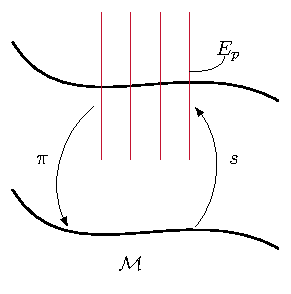
\includegraphics[width=0.4\linewidth]{figures/tikz/section_fiber_bundle.pdf}
\label{img:bspvektorfeld}
\end{figure} 
\end{defs}
\begin{bsp}[Schnitte] \leavevmode
\begin{itemize}
\item Nullschnitt
\begin{align}
&s : \mfk \to E \\
&p \mapsto 0 \in E_p
\end{align}
\item Schnitte von $T\mfk$ heißen Vektorfelder.
Wir bezeichnen die Vektorfelder $V: \mfk \to T\mfk$ mit $\mathfrak{X}(\mfk)$.
\begin{figure}[h]
\centering
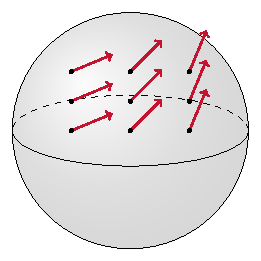
\includegraphics[width=0.4\linewidth]{figures/tikz/vectorfield_on_manifold.pdf}
\caption{Beispiel für ein Vektorfeld}
\label{img:bspvektorfeld}
\end{figure} 
\end{itemize}
\end{bsp}
\begin{satz}
\label{satz:SchnitteModul}
Der Raum der Schnitte $\Gamma (E)$ ist ein Modul über $\mathcal{F}(\mfk)$.
\end{satz}
\begin{bew}[Satz \ref{satz:SchnitteModul}]
Seien $s_1, s_2 \in \Gamma (E)$, so ist $s_1 + s_2 \in \Gamma (E)$
\begin{align}
(s_1 + s_2)(p) := s_1 (p) p s_2 (p)
\end{align}
Sei $\phi \in \mathcal{F}(\mfk), s\in \Gamma(E)$, so ist $\phi \circ s \in \Gamma (E)$
\begin{align}
(\phi \circ s) (p) := \phi (p) s(p).
\end{align}
\end{bew}

\begin{lem}
Sei $(E, \pi, \mfk)$ ein Vektorbündel und $p \in \mfk$.
Dann gilt für alle $x \in E_p$ existiert ein Schnitt $s \in \Gamma (E)$, so dass $s(p)=x$
\end{lem}
\begin{bew}
Wähle eine lokale Trivialisierung von $E$ auf $W \ni p$
\begin{align}
\phi: W \times \R^k \to \pi^{-1}(W) = E\eval_W
\end{align}
und eine glatte Funktion $\varphi \in \mathcal{F}(\mfk)$ mit $\varphi(p)=1$ und $\supp(\varphi) \subset W$.
Sei $\xi \in \R^k$, so dass $\phi (p, \xi)=x$.
Definiere:
\begin{align}
s(q) = \left\{
\begin{array}{ll}
\phi(q, \varphi(q)\xi) & q\in W \\
0_q & q \not\in W \\
\end{array}
\right.
\end{align}
$s$ ist glatt, da folgendes gilt:
\begin{itemize}
\item $s$ ist glatt auf $W$
\item $s$ ist $0$ auf einer Umgebung von $\mfk \setminus W$
\end{itemize}
\begin{align}
s(p) = ( \varphi(p), \varphi(p) \xi ) = \varphi (p \xi) = x
\end{align}
\end{bew}

\begin{defs}[Lokaler Rahmen]
Sei $(E, \pi, \mfk)$ ein Vektorbündel vom Rang $k$ und $U \subset \mfk$.
Ein Rahmen von $E$ über $U$ ist ein $k$-Tupel.
$(s_1, \dots, s_k)$ von glatten Schnitten über $U$ (das heißt $s_i \in \Gamma_i (E)$), so dass für alle $p \in U$
$s_1 (p), \dots, s_k (p)$ eine Basis von $E_p$ bilden.
\end{defs}
	% !TeX root = ..//diffgeo_main.tex
\begin{satz}
\label{satz:lokalrahmentrivialisierung}
Sei $(E, \pi, \mfk)$ ein Vektorbündel vom Rang $k$.
\begin{enumerate}
\item Aus einem lokalen Rahmen folgt eine lokale Trivialisierung.
Sei $(s_1, \dots, s_k)$ ein lokaler Rahmen über $U\subset\mfk$.
Dann ist 
\begin{align}
\phi : U \times \R^k \to E \eval_U\\
(p, \xi) \to \sum^k_{i=1} \xi_i s_i (p),
\end{align}
eine lokale Trivialisierung
\item  Aus einer lokalen Trivialisierung folgt ein lokaler Rahmen.
Sei $\phi: U \times \R^k \to E \eval_U$ eine lokale Trivialisierung.
Dann ist $(s_1, \dots, s_k)$ ein lokaler Rahmen mit 
\begin{align}
s_i(p) = \phi (p, e_i),
\end{align} 
wobei $\{ e_i \}$ die Standardbasis von $\R^k$ ist.
\end{enumerate}
\end{satz}
\begin{bew}[Teil 1 Satz \ref{satz:lokalrahmentrivialisierung}]
Es gilt, dass 
\begin{align}
\phi \eval_p : \{ p \} \times \R^k \to E \eval_p
\end{align}
ein Isomorphismus ist.
Außerdem hat
\begin{align}
\phi : U \times \R^k \to E \eval_U,
\end{align}
maximalen Rang.\\
Für alle $p$ in $U$ existiert eine Umgebung $V \subset U$ von $p$, so dass die folgende Abbildung eine lokale Trivialisierung ist:
\begin{align}
\psi_V : V\times \R^k \to E \eval_V.
\end{align}
Dann gilt:
\begin{align}
\psi^{-1}_V \circ  \phi (q, \xi) = (q, \underbrace{\psi^{-1}_q \circ \phi_q(\xi)}_{\mathrm{Isomorphismus}})
\end{align}
$\psi^{-1}_V \circ \phi : V \times \R^k \to V \times \R^k$ ist ein Diffeomorphismus.
Daraus folgt, dass $\phi$ maximalen Rang auf $V$ und $U$ hat womit folgt, dass $\phi$ ein Diffeomorphismus ist.
\end{bew}
\begin{bew}[Teil 2 Satz \ref{satz:lokalrahmentrivialisierung}]
Diese Aussage ist sofort klar, da $\phi_p$ ein Isomorphismus ist.
\end{bew}

Lokale Rahmen erlauben es uns mit Schnitten zu rechnen.

\begin{defs}[Hauptteil]
Sei $(s_1, \dots, s_k)$ ein lokaler Rahmen und $\phi$ die dazugehörige lokale Trivialisierung.
Ferner sei $s \in \Gamma_U (E)$ über $U \subset \mfk$.
Dann existiert eine glatte Abbildung
\begin{align}
\sigma : U \to \R^k,
\end{align}
so dass
\begin{align}
&s(p) = \sum^{k}_{i=1} \sigma_i (p) s_i(p)\\
&\phi(p, \sigma(p)) = s(p).
\end{align}
$\sigma$ heißt der Hauptteil von $s$ bezüglich $\phi$.
\end{defs}

\begin{bem}
Die Aussagen: $\sigma$ ist glatt und $s$ ist glatt sind äquivalent.\\
Sei $(t_1, \dots t_k)$ ein lokaler Rahmen über $V$ und $\psi$ die dazugehörige lokale Trivialisierung, so dass $U \cap V \neq \emptyset$.
Über $U \cap V$ gilt:
\begin{align}
s_i = \sum_j g^j_i t_j,
\end{align}
wobei $g^j_i : U \cap V \to \R$.
Setze $g(p) = (g^j_i (p))^k_{i,j =1}$
\begin{align}
&g(p)(t_1(p), \dots , t_k(p)) = (s_1(p), \dots, s_k(p))\\
&g: U \cap V \ni p \to g(p) \in \mathrm{GL}(E\eval_p)
\end{align}
sei $s \in \Gamma_{U \cap V} (E)$ und Hauptteile $\sigma_\phi$, $\sigma_\psi$, dann ist
\begin{align}
&\sigma^i_\phi = \sum^k_{j=1} g^j_i \sigma^j_{\psi}\\
&\sigma_\phi = g \sigma_\psi\\
&g : U \cap V \to \mathrm{GL} (k, \R)
\end{align}
\end{bem}


\begin{defs}[Pullback]
Sei $E	\xrightarrow{\pi} \mfk$ ein Vektorbündel und $f : \mfka \to \mfk$ eine glatte Abbildung.
Der Pullback von $E$ über $f$ ist das Vektorbündel $f^* E$ welches definiert ist durch:
\begin{enumerate}
\item $(f^* E)_{p \in \mfka} = \{ (p, x) \vert x \in E_{f(p)}\}$
\item sei $\phi : U \times \R^k \to E\eval_U$ lokale Trivialisierung von $E$
\begin{align}
&f^* \phi : f^{-1} (U) \times \R^k \to (f^* E)\eval_{f^{-1}(U)}\\
&(p, \xi) \mapsto (p, \phi(f(p), \xi)) 
\end{align}
\end{enumerate}
\end{defs}


\begin{defs}
Ein Schnitt von $E$ entlang von $f$ ist eine glatte Abbildung $\delta : \mfka \to E$, so dass $\pi \circ s = f$. 
\end{defs}

\section{Zusammenhang und kovariante Ableitung}

\begin{defs}[Lie-Klammern]
\begin{align}
&\comm{\cdot}{\cdot} : \mathfrak{X}(\mfk) \times \mathfrak{X}(\mfk) \to \mathfrak{X}(\mfk)\\
&\comm{X}{Y} f := X(Y(f)) - Y(X(f))
\end{align}
Hier bleibt als Übung zu zeigen, dass $\comm{X}{Y}$ tatsächlich ein neues Vektorfeld ist.\\
Zusammen mit der Lie-Klammer ist $\mathfrak{X}(\mfk)$ eine Lie-Algebra.
\end{defs}

\begin{defs}[Zusammenhang]
Sei $(E, \pi, \mfk)$ ein Vektorbündel vom Rang $k$.
Ein Zusammenhang auf $E$ ist eine Abbildung
\begin{align}
&\covd : \mathfrak{X}(\mfk) \times \Gamma(E) \to \Gamma (E) \\
&(X, s) \mapsto \covd (X, s) = \covd_X s
\end{align}
Wobei folgende Eigenschaften erfüllt sind:
\begin{enumerate}
\item $\covd$ ist tensoriell in $X$: 
\begin{align}
&\covd_{X_1 + X_2} s = \covd_{X_1} s + \covd_{X_2} s \\
&\covd_{\phi X} s = \phi \ \covd_X s
\end{align}
\item $\covd$ ist eine Derivation in s:
\begin{align}
&\covd_X (s_1 + s_2) = \covd_X s_1 + \covd_X s_2\\
&\covd_X (\phi s) = X (\phi) s + \phi \ \covd_X  s
\end{align}
\end{enumerate}
\end{defs}

Wir führen hier die folgende Notation ein:
$\covd_X s$ heißt die kovariante Ableitung von $s$ in Richtung $X$.\\
\textbf{Wichtiger Spezialfall}:
\begin{align}
&E = T\mfk\\
&\covd: \underbrace{\mathfrak{X}(\mfk)}_{\mathrm{tensoriell}} \times \underbrace{\mathfrak{X}(\mfk)}_{\mathrm{derivativ}} \to \mathfrak{X}(\mfk)
\end{align}

\begin{bsp}
Sei $E = \mfk \times \R^k$ das triviale Bündel mit
\begin{align}
&s: \mfk \to E \\
&p \mapsto (p, \sigma(p))
\end{align}
wobei $\sigma = (\sigma_1, \dots, \sigma_k)$, $\sigma_i \in \mathcal{F}(\mfk)$.
Dann ist der kanonische Zusammenhang gegeben als:
\begin{align}
(\covd_X s)(p) = (p, X_p(\sigma_1), \dots, X_p(\sigma_k))
\end{align}
Wir benutzen die folgende Notation: $\covd_X s = X(\sigma)$.
\end{bsp}

\begin{lem}
\label{lem:lokalisierung1}
$X_1, X_2 \in \mathfrak{X}(\mfk)$ und $X_1(p) = X_2(p)$,
dann folgt daraus, dass 
\begin{align}
(\covd_{X_1} s)(p) = (\covd_{X_2} s) (p).
\end{align}

\end{lem}

\begin{lem}
\label{lem:lokalisierung2}
$s_1, s_2 \in \Gamma(\mfk)$ und $s_1 = s_2$ in einer Umgebung von $p$,
daraus folgt, dass
\begin{align}
(\covd_{X} s_1)(p) = (\covd_{X} s_2) (p).
\end{align}
\end{lem}

\begin{bew}[Lemma \ref{lem:lokalisierung2}]
Wähle $\phi \in \mathcal{F}(\mfk)$ mit $\supp \phi \subseteq U$ und $\phi = 1$ auf einer Umgebung $V \subset U$ von p.
Dann gilt 
\begin{align}
&\phi s_1 = \phi s_2 \\
&\covd_X(\phi s_1)(p) = \covd_X(\phi s_2)(p)
\end{align}
Für die linke Seite ist
\begin{align}
\covd_X(\phi s_1)(p) = \underbrace{X(p)}_{=0} s_1(p) + \underbrace{\phi(p)}_{=1} \covd_X s_1(p) = \covd_X s_1 (p).
\end{align}
Das gleiche gilt für die rechte Seite und somit folgt die Aussage:
\begin{align}
(\covd_{X} s_1)(p) = (\covd_{X} s_2) (p).
\end{align}
\end{bew}

	% !TeX root = ..//diffgeo_main.tex

Als nächstes möchten wir Lemma \ref{lem:lokalisierung1} beweisen.
Allerdings können wir gleich etwas allgemeineres beweisen wodurch Lemma \ref{lem:lokalisierung1} sofort klar ist.

\begin{lem}
\label{lem:tensorielllokalisierung}
Sei $\mathcal{L}: \Gamma (E) \to \Gamma(E')$ eine tensorielle Abbildung. 
Tensoriell bedeuetet hierbei, dass
\begin{align}
\mathcal{L}(\phi s) = \phi \mathcal{L}(s), \quad \forall \phi \in \mathcal{F}(\mfk)
\end{align}
gilt.
Sei weiterhin $p\in \mfk$ und $s, \tilde{s} \in \Gamma(E)$ mit $s(p) = \tilde{s}(p)$, dann gilt
\begin{align}
\mathcal{L}(s)(p) = \mathcal{L}(\tilde{s})(p)
\end{align} 
\end{lem}
Lemma \ref{lem:lokalisierung1} folgt sofort aus diesem Lemma, da die Abbildung
\begin{align}
&\covd_\cdot s : \mathfrak{X}(\mfk) \to \Gamma (E)\\
& x \mapsto \covd_x s
\end{align}
tensoriell ist.

\begin{bew}[Lemma \ref{lem:tensorielllokalisierung}]
Sei $U$ eine Umgebung von $p$ und $\phi = (s_1, \dots, s_k)$ ein lokaler Rahmen auf $U$.
Sei außerdem $\varphi$ eine Bumpfunktion mit $\supp \varphi \subset U$ und $\varphi (p) = 1$.
Wir schreiben 
\begin{align}
s = \sum_{i=1}^k \sigma_i s_i , \quad \tilde{s} = \sum_{i=1}^k \tilde{\sigma}_i s_i
\end{align}
mit $\sigma_i (p) = \tilde{\sigma}_i (p)$.
\begin{align}
\mathcal{L}(s)(p) &= \varphi^2 (p) \mathcal{L}(s)(p)\\
&= \mathcal{L}(\varphi^2 s)(p)\\
&= \sum_{i = 1}^k \mathcal{L}((\varphi \sigma_i)(\varphi s_i)) (p)\\
&= \sum_{i = 1}^k \varphi (p) \sigma_i (p) \mathcal{L}((\varphi s_i)) (p) 
\end{align}
Analog rechnet man mit $\tilde{s}$
\begin{align}
\mathcal{L}(\tilde{s})(p) = \sum_{i = 1}^k \varphi (p) \tilde{\sigma}_i (p) \mathcal{L}((\varphi s_i)) (p) .
\end{align}
Da $\sigma_i = \tilde{\sigma}_i$ und $\varphi(p)=1$ folgt nun die Aussage
\begin{align}
\mathcal{L}(s)(p) = \mathcal{L}(\tilde{s})(p).
\end{align}
\end{bew}

\begin{defs}[Tensorfeld]
Ein Tensorfeld vom Typ $(n, s)$ ist ein glatter Schnitt des Bündels
\begin{align}
T^{n}_{s} (\mfk) = \left( \bigotimes^n_{i=1} T \mfk \right) \otimes \left(\bigotimes^s_{i=1} T^{s*} \mfk\right).
\end{align}
In anderen Worten ist ein Tensorfeld vom Typ $(n,s)$ eine Abbildung
\begin{align}
B : \underbrace{\mathfrak{X}(\mfk) \times \cdots \times \mathfrak{X}(\mfk)}_{s \ \mathrm{mal}} \to \underbrace{\mathfrak{X}(\mfk) \times \cdots \times \mathfrak{X}(\mfk)}_{n \ \mathrm{mal}},
\end{align}
die tensoriell in jedem Argument ist.\\
Lemma \ref{lem:tensorielllokalisierung} sagt uns, dass jede Abbildung $B$ aus einem Vektorfeld kommt.
\end{defs}
An dieser Stelle wollen wir noch einmal kurz einige Fakten über Tensoren sammeln.
Ein Tensor vom Rang $n$ ist:
\begin{align}
t = \sum^n_{i=1} \xi_i \otimes \eta_i
\end{align}
Sei $V$ ein Vektorraum. 
Dann gibt es eine Korrespondenz zwischen
\begin{enumerate}
\item bilineare Abbildung 
\begin{align}
V \times V \to \R
\end{align}
\item Tensoren 
\begin{align}
V^* \otimes V^* = (V \otimes V)^*
\end{align}
\item lineare Abbildungen
\begin{align}
V \otimes V \to \R
\end{align}
\end{enumerate}
wie folgt:
Seien $\xi, \eta \in V^*$ mit $\xi, \eta: V \to \R$.
Dann gibt es die folgende bilineare Abbildung 
\begin{align}
(\xi \otimes \eta)(v, w) = \xi (v) \eta (w).
\end{align}
Allgemeiner hat das Tensorpodukt die folgende Gestalt:
\begin{align}
\left( \bigotimes^n V \right) \otimes \left( \bigotimes^s V^* \right)
\end{align}


Wir kehren nun wieder zu den Tensorfeldern zurück.

\begin{kor}
Sei $B$ ein Tensorfeld vom Typ $(n, s)$, dann induziert $B$ für alle $p$ eine $s$-lineare Abbildung:
\begin{align}
&B_p: T_p \mfk^s \to T_p \mfk^n\\
&(v_1, \dots, \v_s) \mapsto B_p (v_1, \dots, v_s)
\end{align}
\end{kor}
Wir wollen nun wieder zu Zusammenhängen zurückkehren.
\begin{bsp}[Kanonischer Zusammenhang]
Wir wählen die Koordinaten wie folgt:
\begin{align}
s(p) = (p, \sigma(p)), \quad s \in \Gamma(\mfk \times \R^k),
\end{align}
wobei $\sigma = (\sigma_1, \dots, \sigma_k)$ wobei $\sigma_i \in \mathcal{F}(\mfk)$.
Dann ist der kanonische Zusammenhang wie folgt gegeben:
\begin{align}
\covd_x s = (x(\sigma_1), \dots, x(\sigma_k))
\end{align}
\end{bsp}

Sei $\omega$ eine $1$-Form auf $\mfk$ mit Werten in Matrizen $\mathrm{Mat}_{k \times k}(\R)$.
Das bedeutet, dass
\begin{align}
&\omega \in \Gamma(\mathrm{Hom}(T\mfk, \mathrm{Mat}_{k \times k}(\R))) \\
&\omega_p: T\mfk \to \mathrm{Mat}_{k \times k}(\R) \\
&\omega = (\omega{ij})^k_{i,j=1}
\end{align}
$\omega_{ij}$ ist eine $1$-Form auf $\mfk$
\begin{align}
w^{ij}_p :T_p \mfk \to \R.
\end{align}

\begin{defs}
Mit einer $1$-Form kann folgender Zusammenhang definiert werden:
\begin{align}
(\covd^\omega_x s)(p) = (p, x_p(\sigma) + \omega_p(x_p) \sigma(p))
\end{align}
\end{defs}

\begin{satz}
\label{satz:zusammenhangausform}
Sei $(E, \pi, \mfk)$ ein Vektorbündel und $\covd$ ein Zusammenhang auf $E$.
Weiterhin sei $\omega$ eine $1$-Form mit Werten in $\mathrm{Hom}(E, E)$.
Dann ist 
\begin{align}
D^\omega_x s = \covd_x s + \omega(x) s,
\end{align}
ein Zusammenhang auf $E$
\end{satz}
Umgehrt gilt ebenso der folgende Satz:
\begin{satz}
Seien $\covd$ und $\covd'$ zwei Zusammenhänge auf $E$.
Dann definiert 
\begin{align}
\omega(x) s = \covd'_x s - \covd_x s
\end{align}
eine $1$-Form mit Werten in $\mathrm{Hom}(E, E)$.
\end{satz}
\begin{bsp}
Sei $E = \mfk \times \R^k$. 
\begin{align}
\covd^\omega_x s = (p, x_(\sigma) + \omega_p (x_p)\sigma_p)
\end{align}
Aus dem Satz von eben folgt, dass $\covd^\omega_x s$ alle Zusammenhänge auf $E$ sind.
Aus der Lokalisierung folgt
\begin{align}
\phi : U \times \R^k \to E\big\vert_U.
\end{align}
\end{bsp}
Wir stellen uns die Frage wie wir Zusammenhänge mithilfe einer $1$-Form finden können.
Dies ist mithilfe von Zusammenhangsformen bezüglich eines lokalen Rahmens möglich.
Sei $\phi = (s_1, \dots, s_k)$ ein lokaler Rahmen von $E$ über $U$ und sei $x \in \mathfrak{X}(\mfk)$.
Zudem sind $\covd_x s_1, \dots, \covd_x s_k \in \Gamma(E)$.
Diese lassen sich wie folgt darstellen:
\begin{align}
\covd_x s_i = \sum_{i=1}^k \omega_{ij}(x) s_j
\end{align}
Wobei die $1$-Form $\omega_{ij}(x): U \to \R$ glatt und tensoriell in $x$ ist.
Es ist $s = \sum_i \sigma_i s_i$. 
Damit erhält man:
\begin{align}
\covd_x s &= \sum (x(\sigma_i)s_i + \sigma_i + \sigma_i \covd_x s_i)\\
&= \sum_j x(\sigma_j)s_j + \sum_{j=1}^k \sum_{i=1}^k \sigma_i \omega_{ij} s_j\\
&= \sum_j \left[ x(\sigma_j) + \sum:i \sigma_i \omega_{ij}(x) \right] s_j
\end{align}



	% !TeX root = ..//diffgeo_main.tex

Unser nächster Schritt ist es nun die Parallelverschiebung zu definieren.
Auf dem Weg dorthin ist unser erstes Ziel zunächst die kovariante Ableitung von Schnitten längs einer Abbildung zu definieren.
\begin{enumerate}
\item Zu Schnitten längs einer Abbildung:
\begin{align}
\begin{xy}
  \xymatrix@=0.2\linewidth{
          &   E \ar[d]_{\pi} \\
      \mfka \ar[ur]^{s^\text{{\begin{tiny}$\mfka$\end{tiny}}}}  \ar[r]_f  &   \mfk
  }
\end{xy}
\end{align}
Eine Abbildung $s: \mfka \to E$ heißt Schnitt längs $f: \mfka \to \mfk$ falls:
\begin{enumerate}
  \item[i)]  $s^\text{{\begin{tiny}$\mfka$\end{tiny}}}$ ist glatt
  \item[ii)]  Das obere Diagramm kommutiert: $f = \pi \circ s^\text{{\begin{tiny}$\mfka$\end{tiny}}}$
\end{enumerate}
Notation: $\Gamma_f (E)$\\
\textbf{Wichtiger Spezialfall}: $\mfka = I$, das heißt $f$ ist eine Kurve falls $E = T\mfk$
\begin{figure}[H]
\centering
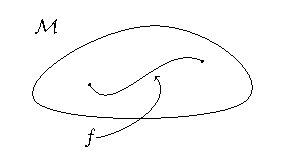
\includegraphics[width=0.4\linewidth]{figures/tikz/curve_on_manifold.pdf}
\label{img:curve_on_manifold}
\caption{Kurve $f$ auf einer Mannigfaltigkeit}
\end{figure} 
Hier sieht das Diagramm dann wie folgt aus:
\begin{align}
\begin{xy}
  \xymatrix@=0.2\linewidth{
          &   T\mfk \ar[d]_{\pi} \\
      I \ar[ur]^{s^I} \ar[r]_f  &   \mfk
  }
\end{xy}
\end{align}
\item Wollen $\covd: \mathfrak{X}(\mfka) \times \Gamma_f (E) \to \Gamma_f (E)$.
\end{enumerate}
\begin{defs}[Kovariante Ableitung längs eines Schnittes]
Sei $\phi = (s_1, \dots, s_k)$ ein lokaler Rahmen von $E$ über $U$ und $s \in \Gamma_f (U)$. 
Dann ist:
\begin{align}
s = \sum^{k}_{i=1} \sigma_i (s_i \circ f)
\end{align}
Dann definieren wir die kovariante Ableitung längs $f$ wie folgt:
\begin{align}
\covd^{f}_x s &= \sum^k_{j=1} \left( x(\sigma_j) + \sum^k_{i=1} \omega_{ij}(f_\ast x)\sigma_i \right) s_j \circ f\\
&= x(\sigma) + (f^\ast \omega)(x) \sigma
\end{align}
Die Wohldefinertheit soll als Übung gezeigt werden.
\end{defs}
\begin{satz}
Die kovariante Ableitung $\covd^f$ längs $f$
\begin{align}
\covd^f: \mathfrak{X}(\mfka) \times \Gamma_f (E) \to \Gamma_f (E),
\end{align}
ist tensoriell im ersten Argument und derivativ im zweiten Argument.
\end{satz}
Wenn wir die Schnitte $\Gamma_f (E)$ mit $\Gamma(f^\ast E)$ identifizieren, dann erhalten wir den zurückgezogenen Zusammenhang
\begin{align}
f^\ast \covd : \mathfrak{X}(\mfka) \to \Gamma(f^\ast E) \to \Gamma(f^\ast E).
\end{align}
\begin{satz}
Sei $s^\text{{\begin{tiny}$\mfk$\end{tiny}}} \in \Gamma(E)$, $q \in \mfka$ und $v\in T_q \mfka$.
Dann gilt:
\begin{align}
\covd^f_v (s\circ f) = \covd_{f^\ast v} s
\end{align}
Die wichtigste Situation ist hierbei der Fall der Kurven also mit $\mfka = I$ und $E = T\mfk$.
%\begin{align}
%\begin{xy}
%  \xymatrix@=0.2\linewidth{
%          &   T\mfk \ar[d]_{\pi} \\
%      c : I  \ar[r]_f  &   \mfk
%  }
%\end{xy}
%\end{align}
Hier gilt nämlich
\begin{align}
\covd_t s := \covd^c_{\pdv{t}} s.
\end{align}
\end{satz}
\begin{bem}
Sei $c$ so gewählt, dass $\dot{c}(t) = 0$, das heißt $c(x)=p$.\\
\textbf{Achtung:} $\covd_t s$ kann ungleich Null sein, selbst wenn $\dot{c}(t) = 0$.
Zum Beispiel: $c(t)=0$ und $s \in \Gamma_c (E)$, dann muss $s(t) \in E_p$ nicht konstant sein.
Dann ist $\covd_t s = \pdv{t} s $ Ableitung um $s(1)$ als Abbildung in $E_p \cong \R^k$.
\end{bem}
Als nächstes wollen wir nun die kovariante Ableitung längs von Kurven verwenden, um die Parallelverschiebung zu definieren.
\begin{defs}[Parallelität]
Sei $c: I \to \mfk$ eine glatte Kurve und $(\pi, E, \mfk)$ ein Vektorbündel.
Ein Schnitt $s^I \in \Gamma_c (E)$ heißt parallel längs $c$ falls 
\begin{align}
\covd^c_t s = 0.
\end{align}
\end{defs}
\begin{figure}[H]
\centering
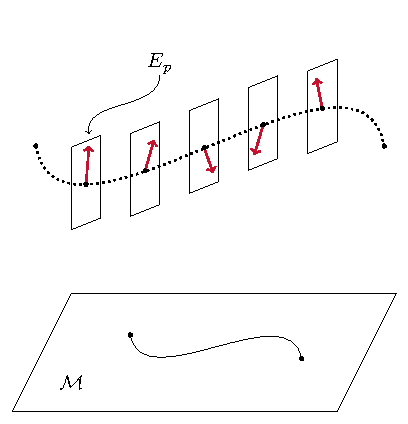
\includegraphics[width=0.7\linewidth]{figures/tikz/parallel_shift_dgl.pdf}
\label{img:parallel_shift:dgl}
\caption{Lösung für die Parallelität auf Vektorbündel}
\end{figure} 
\begin{bem}
Wenn $s_1$ und $s_2$ parallel sind, so sind auf Linearkombinationen $\alpha s_1 + \beta s_1$ ($\forall \alpha, \beta \in \R$) parallel.
\end{bem}
In einem lokalen Rahmen bedeutet $\covd^c_t s = 0$ folgendes:
\begin{align}
\dot{\sigma} + \omega(\dot{c}) \sigma = 0.
\end{align}
Dies ist eine gewöhnliche Differentialgleichung erster Ordnung.
\begin{lem}
Sei $t_0 \in I$ und $x \in E_{c(t_0)}$ dann existiert genau ein paralleler Schnitt $s$ längs $c$ mit $s(t_0 = x)$.
\end{lem}
Sei $c$ eine glatte Kurve mit $c(t_0) = p$ und $c(t_1)=q$ ($t_0, t_1 \in I$).
Setze $P_c(x) = s(t_1)$ wobei $s$ der eindeutig bestimmte parallele Schnitt längs $s(t_0) = x$ ist.
\begin{defs}[Parallelverschiebung]
$P_c : E_p \to E_q$ heißt Parallelverschiebung längs $c$.
\end{defs}
\begin{lem}
\label{lem:BasisVB}
Sei $t_0 \in I$ und seien $s_1, \dots, s_k$ parallele Schnitte längs $c$.
Falls $s^I_1 (t_0), \dots, s^I_k (t_0)$ eine Basis von $E_{c(t_0)}$ ist, so ist $s^I_1 (t), \dots, s^I_k (t)$ eine Basis von $E_{c(t)}$ für alle $t \in I$.
\end{lem}
\begin{bew}[Lemma \ref{lem:BasisVB}]
\begin{align}
s^I_i (t) = Ps^I_i (t_0)
\end{align}
Da $P$ invertierbar ist folgt, dass $s^I_1 (t), \dots, s^I_k (t)$
\end{bew}
\begin{defs}[Paralleler Rahmen]
Ein $k$-Tupel von Schnitten $\phi = (s_1, \dots, s_k)$ längs $c$ heißt Rahmen von $E$ längs $c$, falls $s_1(t), \dots s_k(t)$ eine Basis von $E_{c(t)}$ für alle $t \in I$ ist.
$\phi = (s_1, \dots, s_k)$ heißt paralleler Rahmen, falls alle $s_i$ parallel sind.
\end{defs}
\textit{Warum sind parallele Rahmen für uns interessant?}\\
Wir betrachten den parallelen Rahmen $\phi = (s_1, \dots, s_k)$ und sei $s \in \Gamma_c (E)$.
Das heißt 
\begin{align}
s= \sum^{k}_{i=1} \sigma_i s_i.
\end{align}
Damit erhalten wir für die kovariante Ableitung:
\begin{align}
\covd_t s &= \sum^{k}_{i=1} \covd_t (\sigma_i s_i)\\
&= \sum^{k}_{i=1} (\partial_t \sigma_i) s_i. 
\end{align}
Bezüglich des parallelen Rahmens ist die kovariante Ableitung also gerade die Standardableitung.
\begin{bem}
Parallelverschiebung kann man allgemein längs Stückweiser glatter Kurven $c$ defineren.
\end{bem}



	\chapter{Krümmung}

\begin{defs}[Krümmungstensor]
Der Krümmungstensor eines Zusammenhangs $\operatorname{D}$ auf $E$ ist die Abbildung:
\begin{align*}
\curv: \mathfrak{X}(\mfk) \times \mathfrak{X}(\mfk) \times \Gamma(E) \quad &\rightarrow \quad \Gamma(E) \\
(X, Y, s) \quad &\mapsto \quad \curv(X,Y)s \\
\end{align*}
Hierbei gilt:  \quad $\curv(X,Y)s = \covd_X(\covd_Ys) - \covd_Y(\covd_Xs) - \covd_{[X,Y]}s$
\end{defs}

\textbf{Achtung:} Die Vorzeichen-Konvention ist in der Literatur im Allgemeinen nicht eindeutig!

\begin{satz}
Der Krümmungstensor ist tensoriell in $X, Y$ \& $s$. Außerdem ist er schiefsYmmetrisch in $X$ \& $Y$. 
\begin{bew}
\begin{itemize}
\item $\curv(X,Y) = -\curv(Y,X)$ trivial $\Rightarrow$ SchiefsYmmetrie klar.
\item zu zeigen: $\curv$ ist tensoriell in $s$, das heißt $\curv(X,Y)(\varphi s) = \varphi \curv(X,Y)s$

	\begin{itemize}
		\item[a)] $\covd_X(\covd_Y(\varphi s)) = \covd_X(Y(\varphi)s + \varphi\covd_Ys) = X(Y(\varphi))s + Y(\varphi)\covd_Xs + X(\varphi)\covd_Ys  + \varphi\covd_X(\covd_Ys)$
		\item[b)] $-\covd_Y(\covd_X(\varphi s)) = -Y(X(\varphi))s + -X(\varphi)\covd_Ys - Y(\varphi)\covd_Xs  + \varphi\covd_Y(\covd_Xs)$
		\item [c)] $-\covd_{[X,Y]}(\varphi s) = -[X,Y](\varphi)s - \varphi\covd_{[X,Y]}s$
	\end{itemize}
\end{itemize}
\vspace{.5cm}
$\Rightarrow \curv(X,Y) \varphi s = \varphi \covd_X(\covd_Ys) - \varphi \covd_Y(\covd_Xs) - \varphi \covd_{[X,Y]}s 
= \varphi \curv(X,Y)s $
\end{bew}
\begin{itemize}
\item  zu zeigen: $R$ ist tensoriell in X.
\end{itemize}
\begin{hlem}
$[\varphi X,Y] = \varphi[X,Y] - Y(\varphi) X$
\begin{bew}
$[\varphi X,Y]f = \varphi X(Y(f)) - Y(\varphi X(f)) = \varphi X(Y(f)) - Y(\varphi) X(f) - \varphi Y(X(f))$
\end{bew}
\end{hlem}
\begin{bew}
\begin{align*}
\curv(\varphi X, Y) s &= \covd_{\varphi X} (\covd_Ys) - \covd_Y(\covd_{\varphi X} s) - \covd_{[\varphi X,Y]}s \\
&= \varphi \covd_X (\covd_Ys) - Y(\varphi) \covd_Xs - \varphi \covd_Y(\covd_Xs) - \covd_{\varphi [X,Y]}s + \covd_{Y(\varphi)X}s \\
&= \varphi \curv(X,Y)s
\end{align*}
\end{bew}
\end{satz}
\begin{kor}
$\curv_p: T_p\mfk \times T_p\mfk \times E_p  \rightarrow E_p$ ist punktweise definiert $\forall p \in \mfk$
\end{kor}
\begin{bem}
In vielen Büchern wird zunächst der Fall $E= T\mfk$ diskutiert.
\end{bem}

\begin{bsp}
1) \ Kanonischer Zusammenhang auf $\mfk \times \R^k:$
\begin{align*}
s \in \Gamma(E) \quad \longleftrightarrow \quad \sigma: \mfk \rightarrow \R^k 
\end{align*}
In diesen Fall ist der Krümmungstensor wie folgt gegeben:
\begin{align*}
R(X,Y)s &= \covd_X(\covd_Ys) - \covd_Y(\covd_Xs) - \covd_{[X,Y]}s \\
			&= X(Y(\sigma)) - Y(X(\sigma)) - [X,Y]\sigma \\
			&= 0
\end{align*}
\end{bsp}

\begin{defs}
\begin{itemize}
	\item[a)] Ein Zusammenhang $\covd$ auf $E$ mit $R \equiv 0$ heißt flach.
	\item[b)] Ein Vektorbündel $E$ mit flachem Zusammenhang heißt flaches Bündel.
\end{itemize}
\end{defs}

\begin{bsp}
2) \ Zusammenhang auf $\mfk \times \R^k$ gegeben durch eine $1$-Form mit Werten in $\operatorname{Mat}(k \times k,\R):$
\begin{align*}
\covd^{\omega}_X s &= X(\sigma) + \omega(X)\cdot\sigma \\
							&= \sum_{j=1}^{k} (X(\sigma^{j}) + \sum_{i=1}^{k} \sigma^{i}\omega_i^{\phantom{i}j}(X))s_j \\
							\phantom{.} \\
\curv^{\omega}(X,Y)s &= \covd^{\omega}_X(\covd^{\omega}_Ys) - \covd^{\omega}_Y(\covd^{\omega}_Xs) - \covd^{\omega}_{[X,Y]}s \\
&= \covd^{\omega}_X(Y(\sigma) + \omega(Y)\cdot\sigma) - \covd^{\omega}_Y(X(\sigma)+ \omega(X)\cdot\sigma) - [X,Y](\sigma) - \omega([X,Y]) \sigma \\
\overset{\text{Übung!}}{\phantom{=}} &= X(Y(\sigma)) + X(\omega(Y))\sigma - Y(X(\sigma)) - Y(\omega(X))\sigma + \omega(X)\omega(Y)\sigma - \omega(Y)\omega(X)\sigma - [X,Y]\sigma - \omega([X,Y])\sigma \\
&= \left( \underbrace{X(\omega(Y)) - Y(\omega(X)) - \omega([X,Y])}_{:= \dd\omega(X,Y)} - [\omega(X),\omega(Y)]\right) \sigma
\end{align*}
Hierbei wird $\dd$ äußeres Differential genannt.
\end{bsp}
\textbf{Lineare Zusammenhänge:} $ \quad E= T\mfk$ 
\begin{align*}
\nabla: \mathfrak{X}(\mfk) \times \mathfrak{X}(\mfk) \longrightarrow \mathfrak{X}(\mfk)
\end{align*}

\begin{align*}
\text{\textbf{Krümmung}}:  \qquad \qquad \qquad\curv: \mathfrak{X}(\mfk) \times \mathfrak{X}(\mfk) \times \mathfrak{X}(\mfk) &\longrightarrow \mathfrak{X}(\mfk) \\
\curv(X,Y)Z &= \nabla_X(\nabla_YZ) - \nabla_Y(\nabla_XZ) - \nabla_{[X,Y]}
\end{align*}


\begin{align*}
\text{\textbf{Torsion}:} \qquad\qquad\qquad\qquad\qquad \tor: \mathfrak{X}(\mfk) \times \mathfrak{X}(\mfk) &\longrightarrow \mathfrak{X}(\mfk) \\
(X,Y) &\longmapsto \tor(X,Y) := \nabla_XY -\nabla_YX - [X,Y]
\end{align*}

\begin{lem}
$\tor$ ist tensoriell in $X$ und $Y$.
\begin{bew}
$\tor(X,Y) = -\tor(Y,X)  \longrightarrow$ z.z. $\tor$ tensoriell in $X$. 
\begin{align*}
\tor(\varphi X,Y) &= \nabla_{\varphi X}Y -  \nabla_Y(\varphi X) - [\varphi X,Y] \\
						&= \varphi\tor(X,Y)
\end{align*}
\end{bew}
\end{lem}

\begin{defs}
Ein Zusammenhang $\nabla$ heißt symmetrisch, falls $\tor \equiv 0$.
\end{defs}

\missingfigure{Hier fehlt noch ein kleiner Teil :)}
	% !TeX root = ..//diffgeo_main.tex

\begin{figure}[H]
\centering
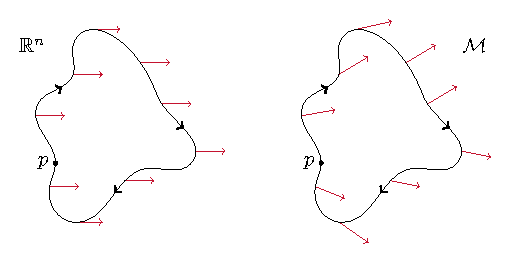
\includegraphics[width=0.7\linewidth]{figures/tikz/parallelshift_rn_vs_manifold.pdf}
\label{img:parallelshift_rn_vs_manifold}
\caption{Parallelverschiebung auf Kurve $c$ in $\R^n$ vs. auf beliebiger Mannigfaltigkeit $\mfk$}
\end{figure} 

Die kovariante Ableitung lässt sich durch Parallelverschiebung ausdrücken.
Wir bezeichnen die Parallelverschiebung entlang $c$ mit $P_c$, wobei $c: (-\epsilon , \epsilon) \to \mfk$ eine Kurve in $\mfk$ ist.
\begin{figure}[H]
\centering
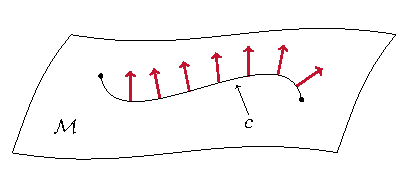
\includegraphics[width=0.5\linewidth]{figures/tikz/parallel_shift_on_curve.pdf}
\label{img:parallel_shift_on_curve}
\end{figure} 
Es gelte $c(0)=p$, $c'(0) = X_p$ und $Y$ sei ein glattes Vektorfeld auf $\mfk$.
Dann gilt:

\begin{align}
\label{eq:parallelcovd}
\nabla_{X_p} Y = \lim\limits_{t \rightarrow 0} \frac{1}{t} \left( P^{-1}_{c(t)} Y_{c(t)} - Y_p\right) 
\end{align}

\begin{bew}[Beweis von Gleichung \ref{eq:parallelcovd}]
Für $Y$, definiert in einer Umgebung von $p_y$, ist der Wert $(\nabla_X Y)(p)$ vollständig bestimmt durch Restriktion von $Y$ auf die Kurve $c$ mit $c'(0) = X_p$.
Expandiere $Y$ als Linearkombination paralleler Vektorfelder längs $c$.

Sei $\{ \hat{w}_1, \dots, \hat{w}_n \}$ eine Basis von $T_p \mfk$.
Sei $w_i : (-\epsilon, \epsilon) \to \mfk$ das parallele Vektorfeld längs $c$ mit $w_i(0) = \hat{w}_i$.
Mit anderen Worten  $\{ w_1(t), \dots, w_n (t)\}$st eine Basis von $T_{c(t)}\mfk$.
\begin{align}
Y = \sum^m_{i=1} a_i w_i
\end{align}
Mit Koeffizienten $a_i: (-\epsilon , \epsilon) \to \R$.\\
Betrachte:
\begin{align}
\lim\limits_{t \rightarrow 0} \frac{1}{t} \left( P^{-1}_{c(t)} Y(t) - Y(0)\right) &=  \lim\limits_{t \rightarrow 0} \frac{1}{t} \left( \sum^m_{i=1} (a_i (t) - a_i (0)) \cdot w_i (0) \right)\\
&= \sum^m_{i=1} \left( \dv{t} a_i (t) \right) \eval_{t=0} w_i (0)\\
&= \covd_t \left( \sum^m_{i=1} a_i w_i \right) \eval_{t=0}\\
&= \nabla_X Y
\end{align}
\end{bew}

\begin{defs}[Parallele Fortsetzung]
Sei $p \in \mfk$ und $v \in T_p \mfk$, dann existiert ein paralleles Vektorbündel längs $c$ mit $X\eval_p = v$.\\
$X\eval_p$ heißt parallele Fortsetzung von $v$.
\end{defs}
Es sellt sich nun die folgende Frage:\\
\textit{Kann man $v \in T_p \mfk$ zu einem parallelen Vektorfeld in einer Umgebung von $p$ fortsetzen?
Also existiert ein Vektorfeld $X$ auf $\mfk$ in einer Umgebung $U$ von $p$, sodass $X\eval_p = v$ und $X$ parallel sind?}
\begin{figure}[H]
\centering
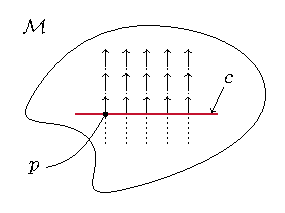
\includegraphics[width=0.6\linewidth]{figures/tikz/parallel_transport.pdf}
\label{img:parallel_transport}
\caption{Paralleltransport}
\end{figure} 
Gegeben sei 
\begin{align}
V: [0, 1] \times [0, 1] \to \mfk\\
(t, \tau) \mapsto V(t, \tau)
\end{align}
Damit erhalten wir ein Vektorfeld $Z$ in einer Umgebung von $p$:
\begin{align}
\label{eq:vectorfieldz}
\nabla_{\pdv{t}} Z \eval_{(t, 0)} = 0, \quad \nabla_{\pdv{\tau}} Z = 0
\end{align}
Wir hätten gerne, dass $\nabla_{\pdv{t}} Z = 0$.
Es genügt zu zeigen, dass folgendes gilt:
\begin{align}
\nabla_{\pdv{\tau}}\nabla_{\pdv{t}} Z = 0
\end{align}
\ref{eq:vectorfieldz} impliziert:
\begin{align}
\nabla_{\pdv{t}}\nabla_{\pdv{\tau}} Z = 0
\end{align}
Es muss deshalb zwangsweise gelten:
\begin{align}
\nabla_{\pdv{t}}\nabla_{\pdv{\tau}} Z - \nabla_{\pdv{\tau}}\nabla_{\pdv{t}} Z = 0.
\end{align}
Da $\comm{\pdv{\tau}}{\pdv{t}} = 0$ gilt, ist 
\begin{align}
R \left( \pdv{\tau}, \pdv{t} \right) Z = 0
\end{align} 
Das bedeutet also falls $\nabla_{\pdv{t}}Z = 0$, dann gilt $R=0$.
Mit anderen Worten $R=0$ ist eine notwendige Bedingung für die Parallelität.
Man kann zeigen, dass $R \equiv 0$ auch hinreichend ist.\\

Betrachte nun die folgende Situation:
\begin{figure}[H]
\centering
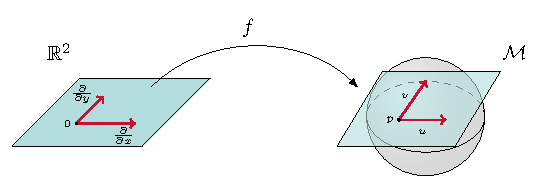
\includegraphics[width=1\linewidth]{figures/tikz/coordinates_r2_manifold.pdf}
\label{img:coordinates_r2_manifold}
\end{figure} 


Sei $f$ glatt und $f(0)=p$ und sei außerdem
\begin{align}
& \dd f \eval_0 \left( \pdv{x} \right) = f_x (0) = u\\
& \dd f \left( \pdv{y}\right) = f_y(0) = v.
\end{align}
Es sei eine Familie von Kurven $c_s$ wobei $0 \leq s \leq 1$ und $c_s (0) = c_s(1) = 0$.
\begin{figure}[H]
\centering
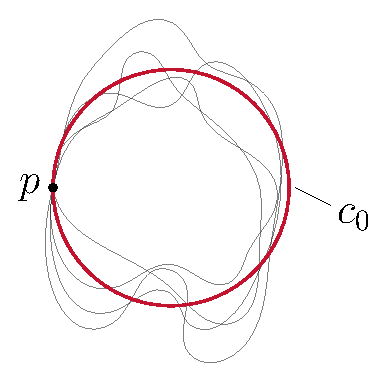
\includegraphics[width=0.4\linewidth]{figures/tikz/variantion_of_closed_curve.pdf}
\label{img:variantion_of_closed_curve}
\caption{Variation der Kurve $c_0$}
\end{figure} 

$P_s$ ist die Parallelverschiebung längs $c_s$.
Wir definieren
\begin{align}
&c : I \times I \to \mfk\\
&(s, t) \mapsto c(s,t)
\end{align}
wie folgt:
\begin{align}
c(s, t) = \left\{
\begin{array}{ll}
f(4 s t, 0) & 0 \leq t \leq \nicefrac{1}{4} \\
f(s, s(4t-1)) & \nicefrac{1}{4} \leq t \leq \nicefrac{1}{2}\\
f(s(3-4t), s) & \nicefrac{1}{2} \leq t \leq \nicefrac{3}{4}\\
f(0, 4s(1-t)) & \nicefrac{3}{4} \leq t \leq 1
\end{array}
\right. 
\end{align}
\begin{satz}
Sei $p \in \mfk$, $u$, $v \in T_p \mfk$ und $f: U \to \mfk$ sei wie oben definiert.
$P_s$ sei die Parallelverschiebung längs $c_s$ von $c_s(0) = p$ nach $c_s(1) = 0$.
Dann gilt:
\begin{align}
\partial_s \partial_s P_s(0) = 2 R (u, v)
\end{align}
\end{satz}

\chapter{Riemannsche Mannigfaltigkeiten}

\section{Wiederholung: Symmetrische Bilinearform}
\begin{defs}[Entartung, Index]
\begin{itemize}
\item Eine symmetrische Bilinearform $B: V \times V \to \R$ ist nicht entartet, falls:
\begin{align}
&B(v, w) = 0, \quad \forall w \in V\\
&\Rightarrow v = 0.
\end{align}
\item $\mathrm{Index}(B) = \max \{ \dim W \vert W \subset V $ ist UR mit $\dim n$ und $B\vert_{W \times W}$ ist negativ definit. $\}$
\end{itemize}
\end{defs}
Es existiert eine Basis ${b_1, \dots b_n}$ von $V_i$, so dass
\begin{align}
c(s, t) = \left\{
\begin{array}{ll}
\hphantom{-} 0 & i \neq j \\
-1 & 1\leq i \leq \mathrm{Index}(B)\\
\hphantom{-} 1 & \mathrm{Index}(B) + 1 \leq i \leq n\\
\end{array}
\right. 
\end{align}
\begin{defs}[Bilinearform zurückholen]
Seien $V$, $W$ $\R$- Vektorräume und $B_V : V \times V \to \R$ eine nicht-entartete symmetrische Bilinearform.
sei außerdem $\phi : W \to V$ eine lineare Abbildung.
Dann ist die zurückgeholte Bilinearform:
\begin{align}
(\phi^\ast B_V) (w_1, w_2) := B(\phi(w_1), \phi(w_2))
\end{align}
\end{defs}
\begin{bem}\leavevmode
\begin{itemize}
\item $(\phi^\ast B_V)$ ist eine symmetrische Bilinearform, die entartet sein kann.
\item Wenn $B_V$ positiv definit und $\phi$ injektiv ist, dann folgt daraus, dass $(\phi^\ast B_V)$ positiv definit ist.
\end{itemize}
\end{bem}

\begin{defs}[Isometrie]
Seien $V$, $W$ $\R$- Vektorräume mit nicht-entarteten Bilinearformen $B_V$ und $B_W$.
$\phi: W \to V$ heißt Isometrie, falls $(\phi^\ast B_V) = B_W$.
\end{defs}

\section{Riemannsche Metriken}

\begin{defs}[Riemannsche Metriken]
Eine (Semi- ) Riemannsche Metrik auf einer differenzierbaren Mannigfaltigkeit $\mfk$, ist eine Familie von nicht-entarteten symmetrischen Bilinearformen 
$(g_p)_{p \in \mfk}$ auf $T_p \mfk$, so dass für alle $X$, $Y$ $\in \mathfrak{X}(\mfk)$ gilt:
\begin{align}
&g_{\cdot} (X_\cdot, Y_\cdot): \mfk \to \R \\
& p \mapsto g_p (X_p, Y_p)
\end{align}
ist glatt in $p \in \mfk$.
\end{defs}


\begin{bem}\leavevmode
\begin{itemize}
\item Eine solche Metrik heißt Riemannsch, wenn $g_p$ positiv definit für alle $p$ in $\mfk$.
\item Eine solche Metrik heißt Lorentz-Metrik, falls $\mathrm{Index} (g_p) = 1$ für alle $p$ in $\mfk$.
\end{itemize}
\end{bem}

\textbf{Zu Semi-Riemannsch}:
Index potentill $\geq 1$, aber auch Riemannsche Metriken werden als Semi-Riemannsch bezeichnet.




	% !TeX root = ..//diffgeo_main.tex

Mittels Riemannscher Metriken lassen sich die wesentlichen geometrischen Eigenschaften von Mannigfaltigkeiten beschreiben.
Sie können verwendet werden um Winkel, Distanz bzw. Längen von Kurven zu messen.

\begin{defs}[(Semi-)Riemannsche Mannigfaltigkeit]
Eine differenzierbare Mannigfaltigkeit $\mfk$ ausgestattet mit einer (Semi-)Riemannschen Metrik $g$, wird (Semi-)Riemannsche Mannigfaltigkeit genannt.\\
\textbf{Notation:} $(\mfk, g)$
\end{defs}

Wir wollen nun (Semi-)Riemannsche Metrik $g$ in lokalen Koordinaten betrachten.
Sei $(x, U)$ eine Karte von $\mfk$.
Ferner bezeichnen wir mit $(X_1, \dots, X_n)$ den dazugehörigen lokalen Rahmen von $T\mfk \eval_U$,
das heißt $X_i = \pdv{x_i}$.
Dann sind 
\begin{align}
g_{ij}: &U \to \R \\
& p \mapsto g_{ij} (p) := g\eval_p (X_i (p), X_j (p))
\end{align}

glatte Funktionen und es gilt:
\begin{align}
g_p \left( X\eval_p, Y \eval_p \right) &= g_p \left( \sum_i^m \xi^i X_j \eval_p, \sum_i^m \eta^i X_i \eval_p \right) \\
&= \sum_{ij} \xi^j \eta^i \underbrace{g\eval_p \left( X_j \eval_p, X_i \eval_p\right) }_{g_{ij}(p)}
\end{align}

\begin{defs}[Fundamentalmatrix]
$(g_{ij})^m_{i, j = 1}$ heißt Fundamentalmatrix von $g$ bzgl. $(x, U)$
\end{defs}

\begin{bem}\leavevmode
\begin{enumerate}
\item Matrix $(g_{ij})^m_{i, j = 1}$ ist symmetrisch, d.h. $g_{ij} = g_{ji}$ (Folgt aus Symmetrie von $g_p$)
\item $(g_{ij})^m_{i, j = 1}$ ist invertierbar (Folgt aus der Tatsache, dass $g_p$ nicht entartet ist)
\end{enumerate}
Die Inverse Matrix von$(g_{ij})^m_{i, j = 1}$ bezeichnen wir mit $(g^{ij})^m_{i, j = 1}$
\end{bem}

\begin{bsp}
\begin{itemize}
\item[a)] Sei $V$ ein reeller $n$-dimensionaler Vektorraum und $\langle\cdot,\cdot\rangle$ eine nicht entartete Bilinearform auf $V$.
Für $v, w \in T_p V$ gilt $g_p (v, w) := \langle v, w \rangle$.
Sei $X: V \to V$ glat ($X$ Vektorfeld), dann gilt
\begin{align}
g_p (X(p), Y(p)) = \langle X(p), Y(p) \rangle
\end{align}
ist glatt.
Daraus folgt, dass $g$ eine Semi-Riemannsche Metrik ist.
Es gilt:
\begin{align*}
g_p \left( \pdv{x_i} , \pdv{x_j} \right) &= \Big{\langle} \phi_p \left(\pdv{x_i}\right) , \phi_p \left( \pdv{x_j} \right) \Big\rangle
&= \langle e_i, e_j \rangle = \delta_{ij}
\end{align*}
\item[b)] Sei $\mfk \subset \R^{n-k}$ eine $n$-dimensionale Untermannigfaltigkeit mit
\begin{align*}
&\phi_p: T_p\mfk \to \R^{n+k}\\
& [c] \mapsto \dv{t} \eval_{t=0} c(t)
\end{align*}
wobei $\phi_p$ injektiv und linear ist.
Dann ist 
\begin{align*}
g_p = \phi^\ast_p \langle \cdot , \cdot \rangle 
\end{align*}
positiv definit.
\begin{defs}
Diese Metrik heißt erste Fundamentalform von $\mfk \subset \R^{n+k}$
\end{defs}
\end{itemize}
\end{bsp}

Als nächstes wollen wir die Existenz von Semi-Riemannschen Metriken zeigen.
\begin{satz}
\label{satz:existenz_metrik}
Jede differenzierbare Mannigfaltigkeit kann mit einer Riemannschen Metrik ausgestattet werden.\\
\textbf{Frage:} gilt dies auch für Semi-Riemannsche Metriken? Übung.
\end{satz}

\begin{bew}[Beweis Satz \ref{satz:existenz_metrik}]
Sei $\{ (x_\alpha, U_\alpha) \}$ Atlas von $\mfk$.
Setze
\begin{align*}
(g_\alpha)_{ij} = \delta_{ij}
\end{align*}
Sei $\varphi_\alpha$ eine glatte Partition der Eins mit $\supp \varphi_\alpha \subseteq U_\alpha$.
Dann setze:
\begin{align*}
g := \sum_\alpha \varphi_\alpha g_\alpha.
\end{align*}
$g$ ist hierbei nach Konstruktion glatt.\\
Positivität: Sei $v \in T_p \mfk$, $v \neq 0$, dann gilt:
\begin{align*}
g_p (v, v) = \sum_\alpha \varphi_\alpha (p) \eval{g_\alpha}_p (v, v) \geq 0.
\end{align*}
Es existiert ein $\alpha_0$, so dass $\varphi_{\alpha_0}(p) > 0$.
\begin{align*}
\Rightarrow g_p (v, v) \geq \varphi_{\alpha_0} (p) \eval{g_{\alpha_0}}_p (v, v) > 0.
\end{align*} 
\textbf{Wichtig:} Wir haben Wahlen getroffen. 
$\Rightarrow$ Metrik $g$ ist nicht kanonisch.
Unter Umständen können Metriken sehr verschiedene Eigenschaften haben.
\end{bew}

Seien $\mfk_1$, $\mfk_2$ differenzierbare Mannigfaltigkeiten und unsere Daten sind jetzt $(\mfk_1, g_1)$, $\mfk_2, g_2$.
\begin{align*}
\phi : \mfk_1 \to \mfk_2, \quad \text{Diffeomorphismus}
\end{align*}
Wir wollen zusätzlich, dass $\phi$ die Metriken erhält, das heißt
\begin{align}
\phi^{\ast} g_2 = g_1
\end{align}
Das heißt vom Standpunkt der Riemannschen Geometrie sind $(\mfk_1, g_1)$ und $(\mfk_2, g_2)$ nicht zu unterscheiden,
wenn $\phi: \mfk_1 \to \mfk_2$ ein Diffeomorphismus mit
\begin{align}
\phi^\ast g_2 = g_1
\end{align}
existiert.
Eine solche Abbildung heißt \textbf{Isometrie}.\\

Unsere nächste Frage ist: wie verhält sich $g_{ij}$ unter Kartenwechsel?
\begin{lem}[Transformationsregel]
\label{lem:Transformationsregel}
Seien $(x, U)$ und $(y, V)$ Karten von $p$.
Dann gilt:
\begin{align*}
g^{y}_{ij} &= g(Y_i, Y_j)\\
&= \sum^m_{k,l = 1} \pdv{y^i}(x^k \circ y^{-1}) \pdv{y^j} (x^l \circ y^{-1}) g^x_{kl}
\end{align*}
\end{lem}
\begin{bew}[Beweis Lemma \ref{lem:Transformationsregel}]
Wir wissen:
\begin{align*}
y_i = \sum^m_{k=1} \pdv{y^i} (x^k \circ y^{-1}) \pdv{x^k}
\end{align*}
Daher gilt:
\begin{align*}
g^y_{ij} &= g(Y_i, Y_j)\\
&= \sum^m_{k,l = 1} \pdv{y^i}(x^k \circ y^{-1}) \pdv{y^j} (x^l \circ y^{-1}) \underbrace{g\left( \pdv{x^l}, \pdv{x^k} \right)}_{= g^x_{lk}}
\end{align*}
\end{bew}

Nächstes Ziel: Führe ausgezeichneten Zusammenhang ein.
Dazu benötigen wir zunächst ein Hilfslemma.
Eine Semi-Riemannsche Metrik $g$ definiert einen Isomorphismus zwischen Tangentialbündel und Kotangentialbündel
\begin{align}
&T \mfk \to T^\ast \mfk\\
&T_p \mfk \ni v \mapsto g_p (v, \cdot) \in T^\ast_p \mfk
\end{align}

\begin{hlem}
\label{hlem:formvfkorrespondenz}
Auf einer Semi-Riemannschen Mannigfaltigkeit $(\mfk, g)$ gibt es eine Eins zu Eins Korrespondenz zwischen Vektorfeldern und $1$-Formen
\begin{align}
&\mathfrak{X}(\mfk) \to \Omega^1 (\mfk)\\
& x \mapsto g(X, \cdot)
\end{align}
\end{hlem}

\begin{bew}[Beweis Hilfslemma \ref{hlem:formvfkorrespondenz}]
Wir haben beweis einen Faserweisen Isomorphismus
\begin{align*}
T_p\mfk \to T^\ast_p \mfk
\end{align*}
definiert.
Zu zeigen bleibt:
glattheit, das heißt $X$ glatt, dass ist $g(X, \cdot)$ glatt.
Arbeite in Karte $(x, U)$, dann ist 
\begin{align*}
\left( \eval{\pdv{x_1}}_p, \dots,  \eval{\pdv{x_m}}_p \right)
\end{align*}
eine Basis von $T^\ast_p \mfk$.
Dann gilt $g_p = \sum g_{ij} \dd{x^i} \otimes \dd{x^j}$.
Das heißt:
\begin{align*}
g_p (X, Y) &= g_{ij} \dd{x^i} \otimes \dd{x^j} \left( \sum \xi^k X_k, \eta^l, X_l\right)\\
&= \sum g_{ij} \xi^k \eta^l \delta_{ik} \delta_{kl}\\
&= \sum g_{ij} xi^i \eta^j
\end{align*}
Wir erhalten als $g(X, Y) = \sum g_{ij}$ für $X= \sum \xi^k X_k$ und $Y= \sum \eta^l Y_l$ beliebig.
Wir schreiben nun auch die $1$-Form in lokale Koordinaten:
\begin{align}
\phi = \sum_j \varphi_j \dd{x^j}
\end{align}
Zu Zeigen: sei $\phi = g(X, \cdot)$ dann sind ide Koeffizientenfunktionen glatt.
\begin{align*}
\phi(Z) &= \sum_j \varphi_j \dd{x^j} \left( \sum \eta^l X_l \right)\\
&= \sum_{j} v\varphi_j \eta^l \dd{x^j} (X_l)\\
&= \sum_j \varphi_j \eta^j
\end{align*}
Nach obiger Rechnung haben wir also:
\begin{align}
\varphi_j = \sum^m_{i=1} g_{ij} \xi^i
\end{align}
dies ist eine glatte Funktion.
\end{bew}

\section{Levi-Civita-Zusammenhang}

\begin{satz}
\label{satz:koszulformel}
Sei $(\mfk, g)$ eine Semi-Riemannsche Mannigfaltigkeit, dann existiert auf $\mfk$ ein Zusammenhang mit den folgenden Eigenschaften:
\begin{enumerate}
\item $\covd$ ist Torsionsfrei:
\begin{align}
\covd_Y X - \covd_X Y = \comm{Y}{X}, \quad \forall X, Y \in \mathfrak{X}(\mfk)
\end{align}
\item $\covd$ ist metrisch:
\begin{align}
X g(Y, Z) = g(\covd_X Y, Z) + g(Y, \covd_X Z), quad \forall X,Y,z \in \mathfrak{X}(\mfk)
\end{align}
\end{enumerate}
Dieser Zusammenhang ist eindeutig durch die \textbf{Koszulformel} bestimmt:
\begin{align}
2 g (\covd_X Y, Z) &= X g(Y, Z) + Y g(X, Z) - Z g(X, Y)\\
&\phantom{=} - g(X, \comm{Y}{Z}) - g(Y, \comm{X}{Z}) + g(Z, \comm{X}{Y})
\end{align}
$\covd$ heißt \textbf{Levi-Civita-Zusammenhang}.
\end{satz}


	\begin{bew}[Beweis Satz \ref{satz:koszulformel}]
Zu zeigen:
\begin{enumerate}
\item Die beiden geforderten Eigenschaften bestimmen den Zusammenhang und Koszuformel ist erfüllt
\end{enumerate}
Die zweite geforderte Eigenschaft impliziert:
\begin{align*}
&X g(Y, Z) = g(\covd_X Y, Z) + g(Y, \covd_X Z)\\
&Y g(X , Z) = g (\covd_Y X, Z) + g(X, \covd_Y Z)\\
&Z g(X, Y) = g(\covd_Z X, Y) + g(X, \covd_Z Y)
\end{align*}
Daraus folgt:
\begin{align*}
X g(Y, Z) + Y g(X , Z) - Z g(X, Y) &= g(\covd_X Y + \covd_Y X, Z) + g(\covd_X Z - \covd_Z X , Y)\\
 & \phantom{=}+ g(\covd_Y Z - \covd_Z Y, X) \\
 &= 2 g(\covd_X Y, Z) - g(\comm{X}{Y}, Z) + g(\comm{X}{Z}, Y) + g(\comm{Y}{Z}, X)
\end{align*}
Damit ergibt sich
\begin{align}
2 g(\covd_X Y, Z) &= g(\comm{X}{Y}, Z) - g(\comm{X}{Z}, Y) - g(\comm{Y}{Z}, X)\\
&\phantom{=} + X g(Y, Z) + Y g(X, Z) - Z g(X, Y)
\end{align}
Definiere  \ $\covd : \mathfrak{X}(\mfk) \times \mathfrak{X}(\mfk) \to \mathfrak{X}(\mfk)$
durch $\covd (X, Y)$, welches das eindeutig bestimmte glatte Vektorfeld ist, das die Koszulformel erfüllt.\\
Es bleibt zu zeigen: \
$\covd : \mathfrak{X}(\mfk) \times \mathfrak{X}(\mfk) \to \mathfrak{X}(\mfk) $ ist ein Zusammenhang.

\begin{enumerate}
\item[1) ] $\covd$ ist tensoriell im ersten Argument:
\begin{align*}
2g(\covd(\varphi X, Y),Z) &= 2g(\covd_{\varphi X}Y, Z) \\
									\phantom{.}\\
									 &= (\varphi X)(g(Y, Z)) + Y(g(\varphi X, Z)) - Z(g(\varphi X, Y)) \\
									 &\phantom{ }- g(\varphi X, [Y, Z])  - g(Y, [\varphi X, Z]) + g(Z, [\varphi X,Y]) \\
									 \phantom{.}\\
									 &= (\varphi X) g(Y, Z) + Y(\varphi)g(X, Z) +(\varphi Y)g(X, Z) \\
									 &\phantom{ }- Z(\varphi)g(X, Y) - (\varphi Z) g(X, Y) - \varphi g(X, [Y, Z]) \\
									 &\phantom{ }-\varphi g(Y, [X, Z]) + Z(\varphi) g(X, Y) - \varphi g(Z, [X, Y]) \\
									 &\phantom{ }-Y(\varphi)g(Z, X)	\\
									 \phantom{.}\\
									 &= \varphi g(\covd_XY, Z)							 
\end{align*}
\item[2) ] $\covd$ ist derivativ im zweiten Argument:
\begin{align*}
2g(\covd_X(\varphi Y), Z) &= X(g(\varphi Y, Z))	+ (\varphi Y) g(X, Z) - Z(g(X, \varphi Y))		\\
										&= g(X, [\varphi Y, Z]) - g(\varphi Y, [X, Z]) + g(Z, [X, \varphi Y]) \\
										\phantom{.}\\
										&= (\varphi X) g(Y, Z) + X(\varphi) g(Y, Z) + (\varphi Y)g(X, Z) \\
										&\phantom{ }- (\varphi Z)g(X, Y) - Z(\varphi)g(X, Y) - \varphi g(X, [Y, Z]) \\
										&\phantom{ }+ Z(\varphi)g(X, Y) - \varphi g(Y, [X, Z]) + \varphi g(Z, [X, Y]) \\
										&\phantom{ }+ X(\varphi)g(Z, Y)\\
										\phantom{.}\\
										&= 2X(\varphi) g(Y, Z) + 2\varphi g(\covd_XY,Z)																										
\end{align*}
\end{enumerate}
\end{bew}

Das nächste Ziel ist die Berechung von $\covd$ in lokalen Koordinaten. Sei also eine Karte $(x, U)$ gegeben. Mit $x_1, \dots, x_n$ bezeichnen wir den zugehörigen lokalen Rahmen. $(x_i = \frac{\partial}{\partial x_i})$
\begin{align}
\covd(x_i, x_j)= \covd_{x_i}^{\phantom{x_i}x_j} = \sum_{k=1}^{m} \Gamma^k_{ij} x_k
\end{align}
Hierbei bezeichnet man $\Gamma^k_{ij}: \mfk \longrightarrow \R$ als \textbf{Christoffel-Symbole}. \\
Sei $\covd$ nun torsionsfrei, das heißt $\covd_XY - \covd_YX = [X, Y]$.
Für $X=x_i$ und $Y=x_j$ gilt $[x_i, x_j]=0$. Damit gilt: 
\begin{align*}
\covd_{x_i}^{\phantom{x_i} x_j} - \covd_{x_j}^{\phantom{x_j}x_i} &= 0 \\
\Longleftrightarrow \quad \sum_{k=1}^{m}\Gamma^k_{ij} x_k - \sum_{k=1}^{m}\Gamma^k_{ji} x_k &= 0\\
\Longleftrightarrow \hspace{1cm} \sum_{k=1}^{m}\left[\Gamma^k_{ij} - \Gamma^k_{ji} \right] x_k &= 0
\end{align*}
Daraus erhalten wir: \ $\Gamma^k_{ij} = \Gamma^k_{ji}$ für den Fall der Torsionsfreiheit. \\
\phantom{.}\\
Sei $\nabla$ der Levi-Civita-Zusammenhang.
\begin{align*}
g(\nabla_{x_i}x_j, x_k) &= \frac{1}{2}\left[x_i(g(x_j, x_k)+ x_j(g(x_i, x_k)) - x_k(g(x_i, x_j)) \right] \\
								 &=  \frac{1}{2}(\partial_i g_{jk} + \partial_j g_{ik} - \partial_k g_{ij})
\end{align*}
\begin{align}
\nabla_{x_i}^{\phantom{x_i}x_j} = \sum_{k=1}^{m}\Gamma_{ij}^k x_k
\end{align}
\begin{align*}
g(\nabla_Xx_j, x_l) &= g\left(\sum_{k=1}^{m}\Gamma_{ij}^k x_k, x_l\right) \\
							&= \sum_{k=1}^{m}\Gamma_{ij}^k \ \underbrace{g(x_k, x_l)}_{g_{kl}}							
\end{align*}
Daraus erhalten wir eine Formel zur Berechnung der Christoffel-Symbole:
\begin{align}
\Gamma_{ij}^k = \frac{1}{2} \sum_{l}g^{kl}\left(\partial_i g_{jl} + \partial_j g_{il} - \partial_l g_{ij}\right)
\end{align}

\chapter{Geodätische}
Geodätische sind Kurven, die das Konzept der Geraden im $\R^n$ auf Mannigfaltigkeiten verallgemeinern.
\missingfigure{Gerade}
\begin{defs}[Geodätische]
Sei $\mfk$ eine Mannigfaltigkeit mit einem linearen Zusammenhang $\nabla$, $I \subseteq \R$ offen. Eine Kurve $c: I \longrightarrow \mfk$ ist eine Geodätische falls:
\begin{align*} 
\nabla_{\frac{\partial}{\partial t}} \dot{c}(t) = 0 \qquad (\nabla_t \dot{c}(t) = 0)
\end{align*}
\end{defs}
 
\textbf{In lokalen Karten:} \\
Sei $(x,U)$ Karte von $\mfk$, \ $c: I \longrightarrow \mfk$ Geodätische. 
\begin{align}
c^k = x^k \circ c: \ I \longleftarrow \R
\end{align}

\begin{align}
\dot{c}(t) = \sum_k \dot{c}^k(t) \eval{\frac{\partial}{\partial x^k}}_{c(t)}
\end{align}

\begin{align*}
0=\nabla_t\dot{c}(t) &= \sum_{k=1}^{m}\nabla_t(\dot{c}^k(x_k\circ c)) \\
							   &= \sum_k \ddot{c}^k(t)(x_k\circ c) + \dot{c}^k(t)\nabla_{\dot{c}(t)}x_k \\
							   &= \sum_k \left(\ddot{c}_k(t) + \sum_{i,j}\dot{c}^{i}\dot{c}^j \Gamma_{ij}^k c(t)\right) x_k \circ c
\end{align*}

Wir betrachten die Kurve $\gamma(t)= \begin{pmatrix}
x(t) \\ y(t) \\z(t) \end{pmatrix}$. \\

Durch auswerten der zuvor hergeleiteten Gleichung erhalten wir:




	% !TeX root = ..//diffgeo_main.tex

HIER FEHLT EINE VORLESUNG

\section{Geodätische}
Eine Gerade im $\R^n$ ist
\begin{align}
&c: I \to \R^n\\
&c(t) = a t + b; \quad a,b\in\R^n
\end{align}
mit $\dot{c}(t)=a$.
Im $\R^n$ ist eine solche Gerade die Geodätische.
Mit einem Zusammenhang können wir dieses Konzept auf Mannigfaltigkeiten verallgemeinern.
\begin{defs}[Geodätische]
Sei $\mfk$ eine Mannigfaltigkeit mit linearen Zusammenhang $\nabla$.
Eine Kurve $c : I \to \mfk$ ist eine Geodätische, falls
\begin{align}
\label{eq:geodätische}
\nabla_t \dot{c} = 0
\end{align}
\end{defs}
Dies ist eine Differentialgleichung, wenn wir in lokale Koordinaten übergehen.
Es sei die Karte $(x, U)$ mit $U \subset \mfk$ und $x: U \to \R^n$ gegeben.
Die Koordinaten sind dann gegeben durch:
\begin{align*}
&x_1 : U \to \R\\
&\vdots\\
&x_k : U \to \R
\end{align*}
mit $x_k = \pdv{x_k}$.
Die Kurve
\begin{align*}
c : I \to U \subset \mfk
\end{align*}
hat die Koordinaten
\begin{align*}
c^k = x^k \circ c\\
\dot{c}(t) = \sum_k \dot{c}^k(t) \pdv{x_k} \eval{c(t)}
\end{align*}
Wir setzen dies in Gleichung \ref{eq:geodätische} ein.
\begin{align*}
\nabla^c_{\pdv{t}} \dot{c} &= \sum_k \nabla^c_{\pdv{t}} (\dot{c}^k (x_k \circ c))\\
&= \sum_k \ddot{c}^k (t) (x_k \circ c) + \dot{c}^k (t) \nabla_{\dot{c}(t)} x_k\\
&= \sum_k \left( \ddot{c}^k (t) + \sum_{ij} \dot{c}^i \dot{c}^j \Gamma^k_{ij} \right) \cdot (x_k \circ c) \\
&= 0 
\end{align*}
Daraus folgt:
\begin{align}
\ddot{c}^k (t) = - \sum_{ij} \dot{c}^i \dot{c}^j \Gamma^k_{ij}
\end{align}
Wir erhalten also eine gewöhnliche Differentialgleichung zweiter Ordnung.
Diese können wir in zwei Gleichungen erster Ordnung umschreiben.
\begin{align}
&\dot{c}^k (t) = \xi^k(t)\\
&\dot{\xi}^k (t) = - \sum_{ij} \Gamma^k_{ij} \xi^i \xi^j
\end{align}
Auf (Semi-) Riemannschen Mannigfaltigkeiten $(\mfk, g)$ erhalten wir die Geodätische mithilfe des Levi-Civita Zusammenhanges.
\begin{bsp}
\begin{enumerate}
\item $(\R^n, g_{\mathrm{Eukl}})$, $\Gamma^k_{ij}= 0$
\begin{align*}
\ddot{c}^k(t) = 0, quad \forall t, k\\
\Rightarrow \dot{c}(t) = \mathrm{const.}\\
\Rightarrow c(t) = a t + b
\end{align*}
\item $(\R^n, g_{\mathrm{Minkowski}})$, $\Gamma^k_{ij}= 0$
\begin{align*}
\Rightarrow c(t) = a t + b
\end{align*}
\end{enumerate}
\end{bsp} 
\begin{lem}
\label{lem:geolinear}
Sei $c: I \to \mfk$ eine Geodätische, dann folgt daraus, dass 
\begin{align}
\tilde{c}(t) = c(\alpha t + \beta), \quad \alpha, \beta \in \R
\end{align}
ebenfalls eine Geodätische ist.
\end{lem}
\begin{bew}[Beweis Lemma \ref{lem:geolinear}]
\begin{align}
&\dot{\tilde{c}}^k = \alpha \dot{c}^k (\alpha t + \beta)\\
& \ddot{\tilde{c}}^k = \alpha^2 \ddot{c}^k (\alpha t + \beta)
\end{align}
\end{bew}
\begin{defs}[Parametrisierung nach der Bogenlänge]
Sei $(\mfk, g)$ eine (Semi-) Riemannsche Mannigfaltigkeit.
Eine Kurve $c: I \to \mfk$ ist
\begin{itemize}
\item parametrisiert nach der Bogenlänge, falls
\begin{align}
g(\dot{c}, \dot{c}) = 1
\end{align}
\item proportional zu Bogenlänge parametrisiert, falls
\begin{align}
g(\dot{c}, \dot{c}) = \alpha > 0, \quad \alpha \mathrm{const.}
\end{align}
\end{itemize}
\end{defs}
\textbf{Übung:} Geodätische sind immer proportional zur Bogenlänge parametrisiert.\\
Wir brauchen lokale Existenz und Eindeutigkeit für unsere Lösungen.
Erinnerung:\\
Sei $O \in J \subset \R$ ein Intervall und
\begin{align*}
\left. \begin{array}{l}
U \subset \R^m\\
V \subset \R^n
\end{array}
\right\} 
\mathrm{offen}
\end{align*}
und $f: J \times U \times V \to \R^n$ glatt.
Dann existiert für jedes $(u, v) \in U \times V$ ein eindeutiges maximales Intervall $I_{u, v} \subset J$, sodass eine eindeutige Funktion
$x_{u,v}: I_{u, v} \to V$ existiert mit:
\begin{align*}
&\dot{x}_{u, v} (t) = f(t, u, x_{u,v}(t))\\
&x_{u, v}(0) = v
\end{align*}
Ferner ist 
\begin{align*}
O = \{ (t, u, v) \in J \times U \times V  \vert t \in I_{u, v}\}
\end{align*}
offen und
\begin{align*}
(t, u, v) \mapsto x_{u,v}(t)
\end{align*}
ist glatt.\\
\textbf{Literaturhinweis:} \textit{Fundamentals of differential geometry} Kapitel 4
\begin{satz}
Sei $\mfk$ ein Mannigfaltigkeit mit dem Zusammenhang $\nabla$
\begin{enumerate}
\item (Existenz) Zu jedem $p \in \mfk$, $v \in T_p \mfk$ existiert ein $I$ und eine Geodätische
\begin{align*}
c: I \to \mfk
\end{align*}
mit $0\in I$, $c(0) = p$, $\dot{c}(0)=v$
\item (Eindeutigkeit) Sind $c_1$, $c_2 : I_i \to \mfk$ Geodätische mit $c_1(0) = c_2(0)$ und $\dot{c}_1 (0) = \dot{c}_2 (0)$, dann folgt:
\begin{align*}
c_1(t) = c_2(t), \quad \forall t \in I_1 \cup I_2
\end{align*}
\item Gegeben $p, v$ dann existiert ein eindeutiges maximal offenes Intervall $I_v \ni 0$ und maximale Geodätische (Also Geodätische auf dem maximalen Intervall)
\begin{align*}
c_v : I_v \to \mfk
\end{align*}
mit $\dot{c}_v (0) = v$ und $c(0)= \pi (v)$
\item Die Menge
\begin{align}
O = \{ (t, v) \in \R \times T \mfk \vert t \in I_v \}
\end{align}
ist offen und 
\begin{align*}
&c: O \to \mfk\\
& (t,v) \mapsto c_v(t)
\end{align*}
ost glatt.
\end{enumerate}
\end{satz}
\begin{defs}[Vollständigkeit]
Ein Zusammenhang auf $\mfk$ heißt vollständig, falls $O = \R \times T\mfk$.
Das heißt alle Geodätischen sind auf ganz $\R$ definiert.\\
Eine (Semi-) Riemannsche Mannigfaltigkeit heißt vollständig falls der Levi-Civita Zusammenhang vollständig ist.
\end{defs}
\begin{bem}
Ist $f: \mfk \to \mfka$ eine Geodätische, dann folgt daraus, dass $f\circ c: I \to \mfka$ eine Geodätische ist
\end{bem}
\begin{bew}
Übung (Hinweis: Isometrien erhalten Christoffel Symbole).
\end{bew}
Sei $\varphi : \mfk \to \mfk$ ein Diffeomorphismus.
Die Menge der Fixpunkte von $\varphi$ ist:
\begin{align}
\fix (\varphi) = \{ p \in \mfk \vert \varphi (p) = p\} 
\end{align}
\begin{satz}
\label{satz:fixpunkte}
Sei $(\mfk, g)$ ein (Semi-) Riemannsche Mannigfaltigkeit  und $\varphi \in \isom (\mfk, g)$.
Sei $p \i \fix (\varphi)$ und $v \in T_p \mfk$ mit $\dd \varphi_p (v) = v$.
Dann hat die Geodätische
\begin{align}
c_v : I_v \to \mfk
\end{align}
die Eigenschaft: $c_v(t) \in \fix (\varphi)$ für alle $t \in I_v$
\end{satz}
\begin{bew}[Beweis Satz \ref{satz:fixpunkte}]
$\varphi \circ c_v (t) = \tilde{c}(t)$ ist eine Geodätische mit
\begin{align*}
&\tilde{c}(0) = \varphi (p) = p\\
&\dot{\tilde{c}}(0) = \dd \varphi (v) = v\\
&\Rightarrow \tilde{c}(t) = v(t), \quad \forall t \in I\\
&\Rightarrow \varphi (c_v(t)) = c_v (t)\\
&\Rightarrow c_v (t) \in \fix (\varphi)
\end{align*}
\end{bew}

\begin{bsp}[Geodätische auf $S^n$]
\begin{align}
S^n = \{ x \in \R^{n+1} \vert \langle x, x\rangle  = 1\} \subset (\R^{n+1}, \langle \cdot, \cdot \rangle_{\mathrm{Eukl}})
\end{align}
Für $u, v \in p^\perp$ gilt:
\begin{align*}
& \langle v, p \rangle = 0\\
& \langle p, v \rangle = 0\\
& \langle p, p \rangle = 1
\end{align*}
Wir haben die Standardmetrik mit:
\begin{align*}
g_p (v, w) = \langle v, w\rangle 
\end{align*}
Sei $A \in O(n+1)$.
\begin{align*}
& A: \R^{n+1} \to \R^{n+1}\\
& v \mapsto A v \\
& S^n \to S^n
\end{align*}
\begin{align*}
g_p (v, w) &= \langle v, w\rangle\\
&= \langle Av, Aw \rangle\\ 
&= g_{A_p} (A_v, A_w)\\
\Rightarrow A \subset \isom (S^n)
\end{align*}
Seien $p \in S^n$ und $v \in T_p S^n = p^\perp$.
$E = \mathrm{span} \{ v, p \} \subset \R^n$ ist eine Ebene.
Sei $A_E : \R^{n+1} \to \R^{n+1}$ die Speigelung an $E$.
Betrachte den Vektor $(p, v, \underbrace{e_3, \dots, e_{n+1}}_{E^\perp})$
\begin{align*}
&A_E (p) = p\\
& A_E (v) = v\\
& A_E(e_i) = - e_i, \quad \forall i
\end{align*}
$A_E \in O(n+1)  \subset \isom (S^n)$.
$\fix (A) = E \cup S^n$ ist ein Kreis.
\begin{align}
&c_v : I_v S^n\\
&c_v(t) = \cos (\alpha t) p + \sin (\alpha t) \frac{v}{\norm{v}}
\end{align}
Mit der Anfangsbedingung $\dot{c}_v (0) = v$ folgt $\alpha = \norm{v}$.\\
Es folgt, dass $S^n$ vollständig ist, da $I_v = \R$
\end{bsp}
\textbf{Übung:} Finde Geodätische für den Hyperbolischen Raum $H^n$




	% !TeX root = ..//diffgeo_main.tex
\begin{satz}
    Eine reguläre Kurve (das heißt $\dot{c}(t)\neq 0 \forall t \in [a, b]$) die stückweise glatt ist, ist eine Gedodätische genau dann, wenn:
    \begin{enumerate}
    \item $c$ ist eine proportional zur Bogenlänge parametrisierte Kurve
    \item Die erste Variation der Bogenlängeverschwindet für jede eigentliche Variation von $c$
    \end{enumerate}
\end{satz}
\begin{bew}
    \begin{enumerate}
        \item Sei $c$ eine Geodätische.
            Daraus folgt, dass $c$ glatt ist und nach der Bogenlänge parametrisiert ist. 
            $\Rightarrow c$ ist regulär und $\nabla_t \dot{c} = 0$. 
            Asu Gleichung für die Variation der Bogenlänge folgt:
            \begin{align*}
                &\dv{s}L(c_s)\eval{s=0} = [g(v(t), \dot{c}(t))]^b_a + \sum_i g(v(t_i), \Delta \dot{c}(t))\\
                &= 0
            \end{align*}
        \item Sei $c$ nach der Bogenlänge parametrisiert und $\partial_s L (0) = 0$ (das heißt $\dv{s}L(c_s)\eval{s=0}=0$) für jede eigentliche Variation von $c$.
            Betrachte $V = \varphi \nabla_t \dot{c}$.
            $V$ ist dann ein stückweise glattes Variationsfeld längs $c$ mit $V(t)=0$ ($t\in [a, t_i) \cup (t_{i + 1}, b]$)
            Bilde eigentliche Variation $c_s$ von $c$ mit Variationsfeld $V$.
            \begin{align}
                \label{eq:sollverschw}
                0 = \partial_s L(0) &= - \int^{t_{i + 1}}_{t_i} g(\varphi \nabla_t \dot{c}, \nabla_t \dot{c}) \dd t\\
                &= - \int^{t_{i+1}}_{t_i} \varphi \norm{\nabla_t \dot{c}} \dd t
            \end{align}
            Daraus folgt, dass $\norm{\nabla_t \dot{c}} = 0$.
            Damit folgt, dass $c\eval{[t_i, t_{i+1}]}$ eine Geodätische ist.
    \end{enumerate}
    Wir wollen nun noch ein Argument angeben, warum Gleichung \ref{eq:sollverschw} verschwindet.
    Setze $f(t_i) = \dot{c}(t_i - 0) - \dot{c}(t_i - 0)$ und betrachte das parallele Vektorfeld $F$ längs $c$.
    Setze $V = \varphi F $ und betrachte die zugehöreige Einparameter Variation von $c$.
    Dann gilt:
    \begin{align*}
        0 &= \partial_s L(0) = g(v(t_i), \dot{c}(t_i - 0) - \dot{c}(t_i - 0))\\
        &= \varphi(t_i) g(f(t_i), f(t_i))
    \end{align*}
\begin{align}
    f(t_i) = \dot{c}(t_i - 0) - \dot{c}(t_i + 0) = 0
\end{align}
\end{bew}
\section{$(\mfk, g)$ als metrischer Raum} 
Ziel sit es jetzt zu zeigen, dass $(\mfk, d)$ ein metrischer Raum ist, wobei $d$ eine geeignet definierte Distanzfunktion ist.
Um dieses Ziel zu erreichen, benötigen wir zunächst ein paar Überlegungen zur Exponentialabbildung.
Die Exponentialabbildung hat die folgende geometrische Eigenschaft.\\
\missingfigure{Exponentialabbildung}
Es ist zu sehen, dass der Strahl $t v$ auf radiale Geodätische $c_v(t) = \exp_p (t v)$ abgebildet.
$\exp_p$ erhält Orthogonalität zu den radialen Richtungen.
Dies nennt man \textbf{radiale Isometrie}.
\begin{lem}[Gaußlemma]
    \label{lem:gaußlemma}
    Sei $p \in \mfk$, $v \in T_p \mfk $ und $c_v(t) = \exp_p(tv)$ auf $[0, b]$ definiert.
    Dann ist $\exp_p$ in einer offenen Umgebung von $\{ tv \vert t\in [a, b] \} \subset T_p \mfk$ definiert und es gilt.
    \begin{itemize}
     \item[a)] $\dd ( \exp_p \eval{t v})(v) = \dot{c}_v(t)$
    \item [b)] Für $\eta \in T_{tv} ( T_p \mfk ) \cong T_p \mfk$ gilt:
    \begin{align*}
        g(d(\exp_p)_{tv} (\eta), d(\exp_{tv})(v)) = g(\eta, v)
    \end{align*}
    \end{itemize}
\end{lem}
\begin{bew}[Beweis Gaußlemma \ref{lem:gaußlemma}]
zu a):
\begin{align*}
    \dd(\exp_p\eval_{tv})(v) &= \dv{s}\eval_{s=0} \underbrace{\exp_p (tv + sv )}_{c_v(t+s)}\\
    &= \dv{s} \eval_{s=0} c_v (t+s) = \dot{c}_v (t)\\
    &= \dot{c}_c (t)
\end{align*}
zu b):\\
Wir können ohne Beschränkung der Allgemeinheit annehmen, dass $t=1$ (da $c_{tv}(1) = c_v (t)$).
Ferner betrachten wir die Variation $H$ von $c_v$:
\begin{align*}
    &H: (-\varepsilon, \varepsilon)\times[0, 1] \to \mfk\\
    & H(s, t) = \exp_p (t(v + s \eta))
\end{align*}
$V(t)$ sei das zugehörige Variationsfeld mit
\begin{align*}
    V(t) = \dv{s} \eval_{s=0} H(s,t)
\end{align*}
Außerdem ist $c_s(t) = \exp_p (t(v+s\eta))$.
\begin{align*}
    &L(c_s) = \sqrt{g(v + s \eta, v + s \eta)}\\
\end{align*}
\begin{align}
    \label{eq:variation1}
\Rightarrow \partial_s L(0) = \frac{1}{\norm{v}}g(v, \eta)      
\end{align}
Wir können $\partial_s L(0)$ auch mittels der ersten Variation der Bogenlänge berechnen.
\begin{align} 
\partial_s L (0) &= \frac{1}{\norm{v}} g(v(t), \dot{c}_v (t))\eval^1_0\\
&= \frac{1}{\norm{v}} (g(v(1), \dot{c}_v (1)) - g(v(0), \dot{c}_v (0)))\\
\label{eq:variation2}
&= \frac{1}{\norm{v}} (g(d(\exp_p)\eval_v (\eta), \dot{c}_v(1)) - g(v(0), \dot{c}_v (0)))
\end{align}
Die Gleichungen \ref{eq:variation1} und \ref{eq:variation2} implizieren die Behauptung, falls
\begin{align*}
    g(v(0),\dot{c}_v (0)) = 0
\end{align*}
ist.\\
Nach a) können wir ohne Beschränkung der Allgemeinheit annhmen, dass $\eta \perp v$ ist (Warum?).
Das heißt:
\begin{align*}
    0 &= g(\eta, v) = g(\eta, \dot{c}_v(0))\\
    &= g(v(0), \dot{c}_v (0))
\end{align*}
\end{bew}

\begin{defs}[Distanzfunktion]
    Seien $p, q \in \mfk$, so ist
    \begin{align}
        \label{eq:distanzfuntion}
        d(p,q) := \inf \{ L(c) \vert c : [a, b]\to \mfk \ \text{Stückweise glatt mit} \ c(a) = p \ \text{und} \ c(b) = q \}
    \end{align}
    die Distanzfunktion.
\end{defs}
\begin{bsp}
Im $\R^2$ wäre die Distanz zwischen den Punkten $p$ und $q$ die Länge der roten Kurve (Gerade) in Abbildung \ref{img:variation}
\begin{figure}[H]
\centering
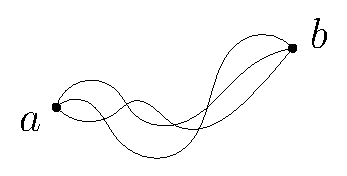
\includegraphics[width=0.3\linewidth]{figures/tikz/variation.pdf}
\caption{Variation}
\label{img:variation}
\end{figure} 
\end{bsp}


\begin{bem}\leavevmode
    \begin{itemize}
        \item Infimum muss nicht angenommen werden (Beispiel: $\R^2 \backslash 0 $)
        \item Die Kürzeste Strecke ist im Allgemeinen nicht eindeutig.
     \end{itemize}
\end{bem}

%appendix
\newpage
\pagenumbering{Roman} %start capital roman numbering for appendices
\pagestyle{plain}

\addcontentsline{toc}{part}{\hfill \Large Anhang}
\part*{Anhang}
\chapter{Wiederholungen und Exkurse}
	\chapter*{A1: Tensoren \& Tensorrechnung}
In diesem Abschnitt seien grundsätzlich alle $V$ endlichdimensionale Vektorräume. \\
\begin{align*}
\mathcal{L}(V_1,\dots, V_k, W) = &\text{ Menge aller multilinearen Abbildungen} \\
&\phantom{ = } V_1 \times V_2 \times \dots \times V_k \longrightarrow W
\end{align*}

\begin{satz}
Für diesen Fall existiert ein Isomorphismus
\begin{align*}
V_1 \otimes \cdots \otimes V_k \cong \mathcal{L}(V_1^*, \dots, V_k^*, \R)
\end{align*}
\end{satz}

\begin{bem}
\begin{align*}
V^{**} &\cong V \\
V_1^* \otimes \cdots \otimes V_k^* &\cong \mathcal{L}(V_1, \dots, V_k, \R)
\end{align*}
\end{bem}

\begin{defs}
Ein kovarianter $k$-Tensor auf $V$ ist ein Element in $\underbrace{V^*\otimes\cdots\otimes V^*}_{\text{k-mal}}$ , das heißt es handelt sich um eine multilineare Abbildung: $ V \times \cdots \times V \longrightarrow \R$
\end{defs}
\textbf{Beispiel:} Die Determinante ist ein kovarianter $k$-Tensor in $\R^k$.
\begin{defs}
Ein kontravarianter $k$-Tensor auf $V$ ist ein Element in $\underbrace{V\otimes\cdots\otimes V}_{\text{k-mal}}$ , das heißt es handelt sich um eine multilineare Abbildung: $ V^*\times \cdots \times V^* \longrightarrow \R$
\end{defs}
Typischerweise treten gemischte Tensoren auf, das heißt Elemente in:
\begin{align*}
\operatorname{T}^{(n, l)}V = \underbrace{V\otimes\cdots\otimes V}_{\text{n-mal}} \ \otimes \  \underbrace{V^*\otimes\cdots\otimes V^*}_{\text{l-mal}}
\end{align*}

\subsubsection*{Tensoren auf Mannigfaltigkeiten}
$\tor^{(r, s)}T\mfk  := \bigsqcup_{p\in\mfk} \tor^{(r, s)}(T_p\mfk)$

\begin{defs}
Ein Tensorfeld vom Typ $(r,s)$ ist ein Schnitt von $\tor^{(r, s)}T\mfk$.
\end{defs}

\textbf{Übung:} Bestimmen sie den Typ der folgenden Tensoren:
\begin{itemize}
\item Vektorfelder
\item $1$-Formen
\item Torsion
\item Krümmungstensor
\end{itemize}	
\section{Explizite Rechnungen in Koordinaten}
	
In diesem Abschnitt wollen wir anhand zweier Beispiele explizite Rechnungen in Koordinaten ausführen. \\
Wir beginnen zunächst mit der Euklidischen Metrik auf $\R^2$:
\begin{align}
g=\dd x^2 + \dd y^2
\end{align}
Wir wollen eine Koordinatentransformation in ebene Polarkoordinaten durchführen:
\begin{align*}
x &\longrightarrow r\cdot \cos\varphi \\
y &\longrightarrow r\cdot \sin\varphi
\end{align*}
Wir erhalten demnach mit Hilfe der Transformationsregel:
\begin{align*}
\dd x &= \frac{\partial x}{\partial r} \dd r + \frac{\partial x}{\partial \varphi} \dd \varphi \\
&= \cos\varphi\dd r - r\sin\varphi\dd\varphi \\
\phantom{.}\\
\dd y &= \sin\varphi\dd r + r\cos\varphi\dd\varphi
\end{align*}
Damit folgt für unsere neue Metrik $g_{\tiny\text{Polar}}$ die Darstellung:
\begin{align*}
g_{\text{Polar}} &= \dd x \otimes \dd x + \dd y \otimes \dd y \\
\phantom{.}\\
&= (\cos\varphi\dd r - r\sin\varphi\dd\varphi) \otimes (\cos\varphi\dd r - r\sin\varphi\dd\varphi) \\ &+ (\sin\varphi\dd r + r\cos\varphi\dd\varphi) \otimes (\sin\varphi\dd r + r\cos\varphi\dd\varphi) \\
\phantom{.}\\
&= \cos^2\varphi \ \dd r \otimes \dd r - r\sin\varphi\cos\varphi \ \dd r \otimes \dd \varphi \\
&- r\sin\varphi\cos\varphi \ \dd \varphi \otimes \dd r + r^2\sin^2\varphi \ \dd\varphi \otimes \dd\varphi \\
&+ \sin^2\varphi \ \dd r \otimes \dd r + r\sin\varphi\cos\varphi \ \dd r \otimes \dd\varphi \\
&+ r \sin\varphi\cos\varphi \ \dd\varphi \otimes \dd r + r^2 \ \dd\varphi \otimes \dd\varphi \\
\phantom{.}\\
&= \dd r \otimes \dd r + r^2 \ \dd\varphi \otimes \dd\varphi
\end{align*}
Die Darstellung der ersten Fundamentalform ergibt sich demnach zu:
\begin{align}
\left(g_{ij}\right)_{\text{Polar}} = 
\begin{pmatrix}
1 & 0 \\
0 & r^2
\end{pmatrix}
\end{align}
\subsection{Christoffel-Symbole}
Wir wollen nun mit dieser Erkenntnis einige Christoffel-Symbole für verschiedene Metriken explizit ausrechnen. \\
Zunächst einmal betrachten wir wieder die \textbf{euklidische Metrik} auf $\R^2$: 
\begin{align*}
g_{ij} = \delta_{ij} = \operatorname{diag}(1,1)
\end{align*}
In diesem Fall verschwinden alle Christoffel-Symbole, da der $\R^2$, allgemeiner auch der $\R^n$ keine Krümmung besitzt, also \textit{flach} ist. WIr erhalten:
\begin{align*}
\Gamma_{ij}^k = 0 \quad \forall i, j ,k
\end{align*}
Dies bedeutet, dass die kovariante Ableitung gleich der "gewöhnlichen"  Ableitung ist, was wir auch erwarten.\\
Kommen wir nun zu der zuvor hergeleiteten Metrik für die \textbf{ebenen Polarkoordinaten}:
\begin{align*}
g= \dd r \otimes \dd r + r^2 \ \dd\varphi \otimes \dd\varphi
\end{align*}
Wir erhalten \ $\frac{\partial}{\partial\varphi} = -y\frac{\partial}{\partial x} +x \frac{\partial}{\partial y}$ \ und damit schließlich:
\begin{align*}
\nabla_{(\frac{\partial}{\partial\varphi})}\frac{\partial}{\partial\varphi}&= \nabla_{(-y\frac{\partial}{\partial x} +x \frac{\partial}{\partial y})}(-y\frac{\partial}{\partial x} +x \frac{\partial}{\partial y}) \\
&=(-y\frac{\partial}{\partial x} +x \frac{\partial}{\partial y})(-y)\frac{\partial}{\partial x} + (-y\frac{\partial}{\partial x} +x \frac{\partial}{\partial y})(x)\frac{\partial}{\partial y} \\
&= -x\frac{\partial}{\partial x} -y\frac{\partial}{\partial x}\\
&= r\frac{\partial}{\partial r}
\end{align*}

Mit diesem Wissen berechnen wir nun explizit die Christoffel-Symbole:
\begin{align*}
\Gamma_{11}^1 &= \frac{1}{2}(1(0+0-0) + 0 \dots) = 0 \\
\Gamma_{11}^1 &= \Gamma_{11}^2 = \Gamma_{12}^1 = \Gamma_{21}^1 = \Gamma_{22}^2 = 0 \\
\Gamma_{12}^2 &= \Gamma_{21}^2 = \frac{1}{2}(r^{-2}\frac{\partial g_{12}}{\partial\varphi} + \frac{\partial g_{22}}{\partial r} - \frac{\partial g_{12}}{\partial\varphi}) = \frac{1}{r} \\
\Gamma_{22}^1 &= -r
\end{align*}

Mit diesem Ergebnis erhalten wir analog wie zuvor:
\begin{align*}
\nabla_{(\frac{\partial}{\partial\varphi})}\frac{\partial}{\partial\varphi} &= \Gamma_{22}^1\frac{\partial}{\partial r} + \Gamma_{22}^2\frac{\partial}{\partial\varphi}\\
&= -r \frac{\partial}{\partial\varphi}
\end{align*}
Zuletzt wollen wir uns eine etwas kompliziertere Metrik auf dem $\R^3$ anschauen:
\begin{align*}
(\R^3, g= (1+x^2)\ \dd x\otimes \dd x + \dd y \otimes \dd y + \e^z \ \dd z \otimes \dd z)
\end{align*}
Daraus folgt direkt für die erste Fundamentalform und ihr Inverses:
\begin{align*}
g_{ij} &= \operatorname{diag}((1+x^2), 1, e^z) \\
g_{ij}^{-1} &= \operatorname{diag}((1+x^2)^{-1}, 1, e^{-z})
\end{align*}
Wir berechnen damit wieder die Christoffel-Symbole mit der bekannten Formel:
\begin{align*}
\Gamma_{ij}^k= \frac{1}{2}\sum_l g^{kl}(\partial_ig_{jl} + \partial_jg_{il}-\partial_lg_{ij})
\end{align*}
Betrachten wir beispielsweise $\Gamma_{12}^3$ fällt auf, dass:
\begin{align*}
\Gamma_{12}^3 &=  \frac{1}{2}\sum_{l=1}^{3} g^{3l}(\partial_1g_{2l} + \partial_2g_{1l}-\partial_lg_{12}) \\
&=  \frac{1}{2}g^{33}(\partial_1g_{23} + \partial_2g_{13}-\partial_3g_{12}) \\
&= 0 \quad \text{, da $g$ diagonal ist.}
\end{align*}
Man findet:
\begin{align*}
\Gamma_{11}^1 &=  \frac{1}{2} g^{11}\underbrace{(2\cdot\partial_1g_{11} -\partial_1g_{11})}_{ = \  \partial_1g_{11} } \\
&= \frac{1}{2} (1+x^2)^{-1}\cdot 2x \\
&= \frac{x}{1+x^2}
\end{align*}
außerdem berechnet man: \quad $\Gamma_{33}^3 = \frac{1}{2}$. \\
\phantom{.} \\
 Alle anderen Christoffel-Symbole sind null!
	\subsection{Parallelverschiebung}
Auch für das in der Vorlesung eingeführte Konzept der Parallelverschiebung wollen wir nachfolgend ein explizites Beispiel liefern. \\
\phantom{.}\\
Sei $\gamma(t)$ die Kurve, die durch die Gleichungen $x = t, y = t$ und $z = t$  definiert wird. Grundlage der Berechnung ist die zuvor bereits verwendete Metrik
\begin{align*}
g= (1+x^2)\ \dd x\otimes \dd x + \dd y \otimes \dd y + \e^z \ \dd z \otimes \dd z)
\end{align*} 
Wie sieht der Paralleltransport entlang $\gamma$ aus? \\

Der Anfangsvektor sei $\left(v_1(0), v_2(0), v_3(0) \right)^T$. Die Formel für den Paralleltransport lautet: 
\begin{align*}
\frac{\dd v(t)}{\dd t} = \sum_{j, k} \Gamma_{jk}^i \frac{\dd x^j}{\dd t} v^k =0
\end{align*}
Komponentenweises Einsetzen unter Berücksichtigung der im vorherigen Abschnitt berechneten Christoffel-Symbole liefert ein System aus drei Differentialgleichungen erster Ordnung:
\begin{align*}
\begin{cases}
\frac{\dd v_1(t)}{\dd t} + \frac{t}{1+t^2}\underbrace{\frac{\dd x}{\dd t}}_{= 1} v_1(t) = 0 \\
\frac{\dd v_2(t)}{\dd t} = 0 \\
\frac{\dd v_2(t)}{\dd t} + \frac{1}{2} \underbrace{\frac{\dd z}{\dd t}}_{= 1} v_3(t)= 0 
\end{cases}
\end{align*}

Die Lösungen dieser Differentialgleichungen ergeben sich zu:
\begin{align*}
	\begin{cases}
		v_1(t) &= \frac{v_1(0)}{\sqrt{1+t^2}}\\
	v_2(t) &= v_2(0) \\
	 v_3(t)& = v_3(0)\e^{-\frac{t}{2}}
	\end{cases}
\end{align*}
Seien $v(0) = \left(v_1(0), v_2(0), v_3(0) \right)^T$ sowie $w(0) = \left(w_1(0), w_2(0), w_3(0) \right)^T$ gegeben, dann gilt für die Vektorfelder, welche durch den Paralleltransport entlang $\gamma$ entstehen:
\begin{align*}
g(v(t),w(t)) = \underbrace{\sum_{i=1}^{3} v_i(0)w_i(0)}_{\text{const.}}
\end{align*}
Es ergibt sich schlussendlich:
\begin{align*}
x g(v,w) = g(\nabla_xv,w) + g(v,\nabla_xw) = 0.
\end{align*}

	\input{content/Exkurs_Geodätische}
	
\addcontentsline{toc}{chapter}{Abbildungsverzeichnis}	
\listoffigures
\end{document}


